\documentclass[zihao=-4,a4paper]{ctexart}
%==================== 数学符号公式 ============
\usepackage{xeCJK}
\newcommand{\zhongsong}{\CJKfontspec{STZhongsong.ttf}}%华文中宋,请自行下载字体并安装
\usepackage{comment}
\usepackage{fontspec}
\setmainfont{Times New Roman}
\usepackage{booktabs}
\usepackage{amsmath}                 % AMS LaTeX宏包
\usepackage[ruled]{algorithm2e}              %伪代码
%\usepackage{amssymb}                % 用来排版漂亮的数学公式
%\usepackage{amsbsy}
\usepackage[style=1]{mdframed}
\usepackage{amsthm}
\usepackage{amsfonts}
\usepackage{mathrsfs}                % 英文花体字 体
\usepackage{bm}                      % 数学公式中的黑斜体
\usepackage{bbding,manfnt}           % 一些图标,如 \dbend
\usepackage{lettrine}                % 首字下沉,命令\lettrine
\usepackage{gbt7714}                 %配置gb7714引用格式

\def\attention{\lettrine[lines=2,lraise=0,nindent=0em]{\large\textdbend\hspace{1mm}}{}}
\usepackage{longtable}
\usepackage[toc,page]{appendix}
\usepackage{geometry}                % 页边距调整
\geometry{top=2.5cm,bottom=2cm,left=2.5cm,right=2cm}
%\usepackage{relsize}                % 调整公式字体大小:\mathsmaller,\mathlarger
%\usepackage{caption2}               % 浮动图形和表格标题样式
\usepackage{booktabs}                %三线表上下加粗
\usepackage{diagbox}                 % 分类表头
%%%使用带圈数字作为教主
\usepackage{pifont}
\usepackage[symbol*,stable]{footmisc}
\DefineFNsymbols{circled}{{\ding{192}}{\ding{193}}{\ding{194}}
{\ding{195}}{\ding{196}}{\ding{197}}{\ding{198}}{\ding{199}}{\ding{200}}{\ding{201}}}
\setfnsymbol{circled}               %带圈脚注
%====================公式按章编号==========================
\numberwithin{equation}{section}
\numberwithin{table}{section}
\numberwithin{figure}{section}
%================= 基本格式预置 ===========================
\usepackage{fancyhdr}
\pagestyle{fancy}
\fancyhf{}  
\fancyhead[C]{\zihao{5}  \songti 武汉理工大学毕业设计(论文)}
\fancyfoot[C]{~\zihao{5} \thepage~}
\renewcommand{\headrulewidth}{0.65pt} 
\ctexset{
    section = {
        format = \centering\zihao{-2} \heiti,
        name = {第, 章}
    },
    subsection = {
        format = \zihao{3} \heiti
    },
    subsubsection = {
        format = \zihao{4} \heiti
    }
}
%================== 图形支持宏包 =========================
\usepackage{subfigure}
\usepackage{graphicx}                % 嵌入png图像
\usepackage{color,xcolor}            % 支持彩色文本、底色、文本框等
\usepackage{hyperref}                % 交叉引用
\usepackage{caption}
\usepackage{amssymb}
\usepackage{bbold}
\usepackage{hyperref}
\hypersetup{
colorlinks=true,
linkcolor=black,
urlcolor=black,
citecolor=black
}
\usepackage{multirow}                  %合并表格
% set up labelformat and labelsep for figure
\captionsetup{labelsep=quad}
\captionsetup{figurewithin=section}

\renewcommand{\thesubfigure}{(\arabic{subfigure})} %还可设置图编号显示格式,加括号或者不加括号
%==================== 源码和流程图 =====================
\usepackage{listings}                % 粘贴源代码
\usepackage{tikz}                    
\usepackage{tikz-3dplot}
\usetikzlibrary{shapes,arrows,positioning}
\usepackage{subfigure}
\usepackage[subfigure]{tocloft}
\renewcommand{\cftsecleader}{\cftdotfill{\cftdotsep}} % 目录后一行连续的点
\renewcommand{\cftsecfont}{\songti{\zihao{-4}}}
\renewcommand{\cftsecpagefont}{\songti{\zihao{-4}}}
\renewcommand\cftdotsep{1}
%===================   正文开始    ===================
\begin{document}
%===================  定理类环境定义 ===================
\newtheorem{example}{例}              % 整体编号
%\newtheorem{algorithm}{算法}
\newtheorem{theorem}{定理}            % 按 section 编号
\newtheorem{definition}{定义}
\newtheorem{axiom}{公理}
\newtheorem{property}{性质}
\newtheorem{proposition}{命题}
\newtheorem{lemma}{引理}
\newtheorem{corollary}{推论}
\newtheorem{remark}{注解}
\newtheorem{condition}{条件}
\newtheorem{conclusion}{结论}
\newtheorem{assumption}{假设}
%==================重定义 ===================
\renewcommand{\contentsname}{~~~~~~~~~~~~~~~~~~~~~~~~~~~~~~~~~~~~~~~~~~~~~~目 ~~ 录}   
\renewcommand{\abstractname}{摘 ~~ 要} 
\renewcommand{\refname}{参考文献}     
\renewcommand{\indexname}{索引}
\renewcommand{\figurename}{图}
\renewcommand{\tablename}{表}
\renewcommand{\appendixname}{附录}
\renewcommand{\proofname}{证明}
\renewcommand{\algorithmcfname}{算法} 
%\renewcommand{\algorithm}{算法} 
%============== 封皮和前言 =================
%===============  封面  =================
\smallskip
\begin{center}

\vspace*{2.2cm}
\zhongsong{\zihao{1} 武汉理工大学毕业设计(论文)} \\
\vspace*{3.3cm}
\heiti{\zihao{2} 基于持续同调的时间序列分类算法}\\
\vspace*{5.5cm}

\zhongsong
\begin{tabular}{cc}
 \zihao{3} 学院(系):&\underline{\makebox[7cm][c]{\zihao{3}数学与统计学院}} \\ 
 \\
 \zihao{3}专业班级: & \underline{\makebox[7cm][c]{\zihao{3}信计2102班}} \\ 
 \\
 \zihao{3}学生姓名: & \underline{\makebox[7cm][c]{\zihao{3}陈凯鑫}} \\ 
 \\
 \zihao{3}指导教师: & \underline{\makebox[7cm][c]{\zihao{3}彭宁宁}} \\ 
 \\
\end{tabular} 
\end{center}
\thispagestyle{empty}
\clearpage
%=====================原创性声明===========
\begin{center}
\zihao{-2} \textbf{学位论文原创性声明}
\end{center}

本人郑重声明:所呈交的论文是本人在导师的指导下独立进行研究所取得的研究成果。除了文中特别加以标注引用的内容外,本论文不包括任何其他个人或集体已经发表或撰写的成果作品。本人完全意识到本声明的法律后果由本人承担。 
\begin{flushright}
\zihao{4} 作者签名:\qquad ~~~\\

年\qquad 月\qquad 日
\end{flushright}
\vskip 2cm
\begin{center}
\zihao{-2} \textbf{学位论文版权使用授权书}
\end{center}

本学位论文作者完全了解学校有关保障、使用学位论文的规定,同意学校保留并向有关学位论文管理部门或机构送交论文的复印件和电子版,允许论文被查阅和借阅。本人授权省级优秀学士论文评选机构将本学位论文的全部或部分内容编入有关数据进行检索,可以采用影印、缩印或扫描等复制手段保存和汇编本学位论文。\smallskip

本学位论文属于
\begin{tabular}[t]{l}
1、保密$ \Box$,在~~~年解密后适用本授权书  \\ 
2、不保密$ \Box$  \\ 
\end{tabular} \\
\begin{center}
(请在以上相应方框内打“$\surd”$)
\end{center}
\begin{flushright}
\zihao{4} 作者签名:  \quad\quad\quad\quad 年 \quad  月  \quad  日\\
导师签名:   \quad\quad\quad\quad 年 \quad  月 \quad   日\\
\end{flushright}
\thispagestyle{empty}
\clearpage

%%=============设计(论文)任务书===========
%\begin{center}
%\zihao{-2}\textbf{\songti 本科生毕业设计(论文)任务书} 
%\end{center}
%\smallskip
%\renewcommand{\arraystretch}{1.3}
%\begin{tabular}{lll}
%\zihao{4} \textbf{\songti 学生姓名: 曹宇} & & \zihao{4} \textbf{\songti 专业班级:\quad\quad 船海1006班} \\ 
%\zihao{4} \textbf{\songti 指导教师:徐海祥}&\makebox [3cm] & \zihao{4} \textbf{\songti 工作单位:\quad 武汉理工大学} \\ 
%\end{tabular}\\
%\begin{tabular}{lll}
%\zihao{4} \textbf{\songti 设计(论文)题目:}& \zihao{4} \textbf{\songti  武汉理工本科论文\LaTeX 模板 } &\\ 
%\zihao{4} \textbf{\songti 设计(论文)主要内容:} \\
%\end{tabular} \\ 
%\begin{enumerate}
%\item \LaTeX 环境的配置
%\item 主要字体的控制和数学公式的选用
%\item 图表和代码的粘贴
%\end{enumerate}
%\begin{tabular}{ll}
%\zihao{4} \textbf{\songti 要求完成的主要任务:}
%\end{tabular} \\ 
%\begin{enumerate}
%\item 选择合适的\TeX 编辑系统
%\item 学习如何使用控制代码完成排版
%\item 合理的安排学习和科研的时间来发展自己兴趣爱好
%\end{enumerate}
%\begin{tabular}{ll}
%\zihao{4} \textbf{\songti 必读参考资料:}
%\end{tabular}
%\begin{enumerate}
%\item \LaTeX  \quad User Manual
%\item  字体设计的艺术
%\end{enumerate}
%\begin{tabular}{lll}
%\zihao{4} \textbf{\songti 指导教师签名: }&\makebox [4cm]& \zihao{4} \textbf{\songti 系主任签名:} \\
%& & \zihao{4} \textbf{\songti 院长签名(章)}
%\end{tabular}
%\thispagestyle{empty}
%\clearpage
%%==========本科生毕业设计(论文)开题报告  =============
%\begin{center}
%\zihao{-2} \textbf{\songti 武汉理工大学}\\
%\zihao{-2} \textbf{\songti 本科生毕业设计(论文)开题报告} 
%\end{center}
%\begin{tabular}{|l|}
%\hline \rule[-2ex]{0pt}{5.5ex} \makebox[13.5cm][l]{\zihao{4} \heiti 1、目的及意义(含国内外的研究现状分析) } \\ 
%\quad \LaTeX 是国际通行的科技论文排版软件,国际上科研机构和大学都采用它写作\\
%\quad 国内著名高校都有自己的本科生\LaTeX 模板供毕业生使用\\
%\quad 但是武汉理工大学还没有本科生\LaTeX 模板可以参考\\
%\quad 人类的价值在于创造而不是索取 \\
%\hline \rule[-2ex]{0pt}{5.5ex}  \zihao{4} \heiti
%2、基本内容和技术方案\\ 
%\quad 采用GITHUB托管降低代码维护成本\\
%\quad 加入在线\TeX 编辑器的使用简介 \\
%\quad 授人以渔,注重方法和理念的引导\\
%\hline \rule[-2ex]{0pt}{5.5ex}  \zihao{4} \heiti
%3、进度安排 \\ 
%\quad 离 deadline 两个月吃喝玩乐 \\
%\quad 离 deadline 一个月吃喝玩乐 \\
%\quad 离 deadline 半个月吃喝玩乐 \\
%\quad 离 deadline 一个星期狂写论文 \\
%\hline \rule[-2ex]{0pt}{5.5ex} \zihao{4} \heiti
%4、指导教师意见 \\ 
%\quad 曹宇同学是个好同志\\
%\quad 曹宇同志是个好同学\\
%\quad 本表格是支持跨页的长表格,你可以复制上面的内容进行测试\\
%\quad 具体方法是将tabular改为 longtable然后再编译\\
%\makebox[10cm][r]指导教师签名:\\
%\makebox[12cm][r]\quad 年\quad 月\quad 日\\
%\hline 
%\end{tabular} 
%\thispagestyle{empty}

\pagestyle{plain}
\pagenumbering{Roman}
\section*{\zihao{-2} \centering 摘 ~~ 要}
% 生成序号列表
 \begin{enumerate}
 \item 简述时间序列分类的重要性以及传统方法的局限性
 \item 引入拓扑数据分析作为一种新兴方法,在捕捉数据内在结构方面的独特潜力
 \item 明确核心:深入综述和比较分析点云构造策略和从PD中提取有效特征的技术
 \item 概述综述的主要内容,对不同方法的原理,优缺点,参数影响和适用性进行比较
 
 \end{enumerate}





\vskip0.5cm

{\zihao{4} \heiti 关键词: } \zihao{-4}拓扑数据分析,时间序列分类,持续同调,点云构造,时间延迟嵌入,特征提取,持久性图
% \addcontentsline{toc}{section}{摘要}

\clearpage
\section*{\zihao{-2} \centering \textbf{Abstract} }
   %用了Times New Roman字体来美化观感
   
here is English Abstract

\vskip0.5cm

\textbf{\zihao{4} Key Words:} Multi-Agent Deep Reinforcement Learning, Formation Control, Path Planning
% \addcontentsline{toc}{section}{Abstract}





\pagestyle{empty}
\tableofcontents
\thispagestyle{empty}
%============== 论文正文   =================
\pagestyle{fancy}



\pagenumbering{arabic}
\section{绪论}
\subsection{研究背景与意义}
在数据挖掘和机器学习中,时间序列的早期分类受到了极大的关注,因为它可以解决包括医疗,工业和运输在内的许多领域的时间关键问题。
文献表明时间序列的早期分类有着很多的应用,以下进行详细讨论:

\begin{itemize}
    \item \textbf{行为分类}: 随着智能手机和可穿戴设备中多模态传感器的可用性,人们可以轻松监控他们的日常活动,
    如步行,跑步,饮食等。人类活动的早期分类有助于最大限度地减少系统的响应时间,
    从而改善用户体验[8]。[8]中的研究人员试图使用MTS生成的传感器对各种复杂的人类活动进行分类,
    例如坐在沙发上、坐在地板上、站着说话、上楼和吃饭。[37]-[39]中的研究集中在识别人类动作,如捡起,小鸡舞,高尔夫挥杆等
    \item \textbf{医疗诊断}:[3]、[43]-[46]、[46]-[51]工作的主要动机是开发哮喘、病毒感染、异常心电图等疾病的早期医学诊断分类方法。
    这些疾病的早期诊断可以显着减少对患者健康的影响并协助医生进行治疗。基因表达已用于研究患者的病毒感染、
    疾病的药物反应和患者恢复[43]-[45]。早期发现哮喘有助于预防危及生命的风险,并进一步提供快速缓解[49]。
    [51]中的研究侧重于使用体温和呼吸频率等生理测量的MTS来预测将患者转移到重症监护室(ICU)的正确时间。
    此外,ECG也是由心脏活动产生的电信号的时间序列。ECG的早期分类[3],[46],[47],[52]有助于最早诊断心脏跳动异常,降低心力衰竭的风险。
    \item \textbf{工业过程监控}:随着传感器技术的进步,通过使用传感器监测工业过程变得方便和轻松。传感器产生时间序列,该时间序列被分类以了解操作的状态。[29],[35],[42],[53]-[56]中的作者致力于通过使用传感器数据来构建基于早期分类的工业问题解决方案。在化学工业中,即使是轻微的泄漏也会对船员的健康造成危险影响[29]。早期分类不仅降低了健康风险,还通过确保始终平稳运行来最大限度地降低维护成本。特别地,在[29]中使用气体传感器开发了电子鼻,以闻到气体气味。它会生成MTS,需要尽早对其进行分类,以检测任何泄漏。在[42]中,作者试图检测液压系统中的泵泄漏、压力降低和操作效率低下等问题。及早发现这些问题可以显著降低维护成本。核电厂仪表故障的早期识别可以避免危险后果[35],[56],[57]。

\end{itemize}

为应对这一需求,研究者不断探索新型特征表示方法,其中基于拓扑数据分析(Topological Data Analysis, TDA)的持续同调技术正逐渐成为突破传统方法瓶颈的重要方向。其基本思想在于利用持续同调捕捉时间序列中的拓扑不变性特征,进而揭示数据背后隐藏的全局结构规律。与传统统计或深度学习方法相比,基于持续同调的方法具有多项显著优势:

\begin{itemize}
    \item 强鲁棒性: 拓扑特征对噪声和尺度变化不敏感,能够有效克服局部波动的干扰。例如,在机械振动信号中,持续同调能够稳定识别出轴承早期故障所对应的环状拓扑模式,而传统的频域分析则容易受到随机噪声的影响。
    \item 结构解释性强: 通过持续同调条形码,可以直观地呈现数据中的关键拓扑模式(如 H1 环状结构和高维空洞),从而增强分类过程的可解释性。在医疗研究中,癫痫 EEG 信号中的短暂高频振荡现象,往往可通过 H1 条形码的突然延长被精准捕获。
    \item 多尺度分析能力: 结合时间延迟嵌入与子窗口分割技术,该方法可同时捕捉长期趋势与瞬时动态。例如,加州大学团队提出的滑动窗口持续同调方法成功检测出了电力负荷序列中的周期性异常。
\end{itemize}

综上所述,基于持续同调的时间序列分类技术对实际应用具有重要意义。它不仅能够帮助工业设备在复杂工况下实现故障早期预警,如在风力发电机振动监测中识别叶片裂纹;在医疗领域,该技术能够辅助诊断阿尔茨海默症患者的脑电信号异常;在智慧城市建设中,还能通过分析交通流量序列的周期性拥堵特征来优化路网规划。未来,随着拓扑数据分析理论和边缘计算技术的不断进步,该方法将推动工业物联网、精准医疗等领域的智能化升级,为复杂系统的决策提供更加可靠的理论支撑。



\subsection{拓扑数据分析简介及其应用于时间序列的动机}
在时间序列分类领域,研究者们提出了多种方法来提高分类性能。以下是一些主要的研究方向和方法:基于形状的方法,基于结构的方法,基于区间的方法,基于集成的方法,基于深度学习的方法.

基于形状的方法主要在于寻找能够区分不同类别的局部模式和子序列。形状方法试图从时间序列中提取局部具有判别性的形状特征,这些特征往往可以直接反映数据中关键的模式变化,从而实现分类。例如,通过比较时间序列中是否存在某个特定的形状(如上升或下降趋势、周期性波动等)来判断类别。
结构方法更侧重于捕捉时间序列的全局或整体特性,如整体趋势、周期性、平稳性等。它们可能通过建立全局模型(如自回归模型、状态空间模型)来描述数据的内在结构,或者利用全局距离度量(如DTW)比较序列的相似性。这类方法强调数据整体形态的结构信息而非局部细节。
区间方法则通过从时间序列中划分出若干个子区间,分别提取区间内的统计特征(如平均值、方差、峰值等),然后利用这些特征构建分类器。这种方法的优势在于可以捕捉到不同时间段内表现出不同统计规律的信息,尤其适用于序列中存在明显局部变化或阶段性特征的情况。
集成方法综合了多种单一分类器或特征提取方法的优势,通过组合多个模型(例如集成形状、区间和结构信息的多个模型),来提高整体分类准确率和鲁棒性。这种方法通常能够抵消单一模型的偏差,并在面对复杂多样的数据时展现出更好的泛化能力。
深度学习方法通过构建多层神经网络(如CNN、RNN、Transformer等),自动从原始数据中学习特征表示,无需人工设计特征。这类方法在大规模数据和复杂模式识别任务中表现突出,能够捕捉到数据中的非线性关系和多尺度信息,但同时也需要更多的数据和计算资源。下面我将介绍一下国内外的研究现状。

Bagnalla 等人 (2017) 对当前时间序列分类方法进行了系统性的综述和广泛的实验评估,涵盖了来自 UCR 存档的 85 个数据集上的 18 种先进算法。他们的研究不仅表明了简单的基线方法(如基于 DTW 的 1-最近邻方法)在很多情况下依然具有竞争力,而且强调了结合多种表示方式的集成方法在性能上具有显著优势。该工作为国内外时间序列分类的研究提供了重要的参考依据,推动了该领域标准化评估方法的建立,也为后续算法的改进和新方法的探索奠定了坚实的实验基础。
Chen 和 Ng (2004) 在他们的论文《On the marriage of Lp-norms and edit distance》中提出了一种将Lp范数和编辑距离相结合的统一框架,详细探讨了如何利用两者的优点来度量序列之间的相似性。他们的研究展示了通过结合连续的Lp距离度量与离散的编辑操作,可以更准确地反映字符串或序列数据的结构特征,为大规模数据检索和序列比较提供了理论支持。该工作在国际数据库大会上发表,为后续在文本、DNA序列等领域的相似性分析方法研究提供了重要的参考。
Marteaup (2009) 提出了一种改进的时间弯曲编辑距离方法,通过引入刚性调节参数来平衡匹配过程中的灵活性和约束性,从而更好地适应时间序列数据中的局部形变。该方法在传统编辑距离的基础上,结合了动态时间规整的思想,能够有效处理因时间扭曲、局部缩放等因素引起的匹配误差问题。实验结果表明,这种方法在模式匹配和相似性搜索任务中不仅提高了匹配准确率,同时保持了较低的计算复杂度,为时间序列匹配领域提供了一种具有较高实用价值的解决方案。
Stefana、Athitsos 和 Dasg (2013) 在他们发表于 IEEE Transactions on Knowledge and Data Engineering 的论文中提出了 Move-Split-Merge (MSM) 距离度量方法。该方法通过引入“移动”、“分割”和“合并”三种基本操作,扩展了传统编辑距离的思想,从而更灵活地处理时间序列数据中的局部非线性变形问题。相比于传统的动态时间规整(DTW)等距离度量,MSM 能够在保留序列局部结构信息的同时,更准确地衡量序列之间的相似性。实验结果表明,MSM 在时间序列分类和相似性搜索任务上表现出更高的鲁棒性和准确性,为时间序列数据挖掘提供了一种有效的新工具。
Schäfer (2015) 在其发表于 Data Mining and Knowledge Discovery 的论文中提出了 BOSS 方法,专注于解决噪声环境下的时间序列分类问题。该方法通过对时间序列数据进行符号化处理,有效地提取出对分类任务具有判别力的特征,同时增强了对噪声的鲁棒性。实验结果表明,在存在较高噪声干扰的情况下,BOSS 能够显著提升分类准确率,为噪声环境下的时间序列分析提供了一个高效且稳健的解决方案。
Schäfer 和 Leser(2017)在他们的论文中提出了 WEASEL 方法,这是一种基于模式袋(bag-of-patterns)思想的快速且准确的时间序列分类方法。该方法利用滑动窗口、傅里叶变换以及统计特征选择相结合的策略,将原始时间序列转换为简洁且具有判别力的符号特征向量,从而实现高效的分类。大量在标准数据集上的实验表明,WEASEL 不仅在分类精度上具有竞争力,而且计算复杂度远低于传统方法,使其在大规模时间序列分类任务中具有较高的实用价值。该研究成果发表于 2017 年 ACM 信息与知识管理会议,为时间序列分类领域提供了一种有效且高效的解决方案。
Morrill 等人(2023)提出了一种基于广义签名(generalised signature)的多变量时间序列特征提取方法。该方法扩展了传统签名变换,旨在捕捉多变量时间序列中各维度之间的交互和时序信息,从而生成具有丰富描述力的特征表示。这篇预印本在理论上探讨了广义签名的数学性质,并通过一系列实验验证了其在下游任务(如分类和回归)中的鲁棒性和有效性。该工作为处理高维、多变量时间序列数据提供了一种新颖且具有竞争力的特征提取工具。
Cabellon 等人提出了一种基于监督区间搜索的时间序列分类方法,旨在提高分类的速度和准确性。他们的方法核心在于自动识别时间序列中最具判别力的区间,并利用监督信号来优化区间选择过程,而不是直接对整个序列进行分析。这样既能捕捉到关键局部特征,又能大幅降低计算开销。实验结果表明,该方法在多个标准数据集上均取得了与最先进算法相当甚至更优的分类效果,同时在运行效率上也有明显优势,为实际应用提供了有力支持。
lynn、Large 和 Bagnall(2019)在论文中提出了 Contract Random Interval Spectral Ensemble (c-RISE) 方法,该方法探讨了在构建集成分类器过程中对区间进行“压缩”处理对分类准确率的影响。具体来说,c-RISE 方法通过随机区间划分和频谱特征提取,将原始时间序列划分为多个局部区间,并对这些区间进行特征压缩,进而构建一个多样化且高效的集成分类器。实验结果表明,采用这种压缩策略不仅能降低模型复杂度和计算成本,同时在多数数据集上提升了分类准确性和鲁棒性。该研究为时间序列分类中如何在保证关键信息的同时减小模型规模提供了新的思路,并为后续相关方法的发展奠定了理论和实践基础。
Middlehurst 等人(2021)在《Machine Learning》期刊上发表的论文中提出了 HIVE-COTE-2.0,一种新型的元集成方法,用于时间序列分类。该方法融合了多种不同类型的分类器(例如基于距离、基于区间、基于形状等),构建了一个统一的分类框架,从而在准确性和鲁棒性方面实现了显著提升。与前一代 HIVE-COTE 方法相比,HIVE-COTE-2.0 不仅在实验中展示了更高的分类准确率,同时也在计算效率上有所改善。这项工作为时间序列分类领域提供了一个创新的、具有竞争力的解决方案,并为未来元集成方法的进一步研究奠定了坚实的理论和实践基础。
Shifaz 等人(2020)在他们发表于 Data Mining and Knowledge Discovery 的论文中提出了 TS-CHIEF 算法,这是一种针对时间序列分类的可扩展且准确的森林算法。该方法通过构建多棵决策树的集成,利用随机特征抽样和专门设计的时间序列转换技术,能够捕捉到时间序列中的关键模式和局部特征。TS-CHIEF 在保持较高分类准确率的同时,也显著降低了计算复杂度,使其能够高效处理大规模数据集。实验结果显示,该算法在多个标准数据集上的表现均优于或相当于现有最先进的时间序列分类方法,为实际应用和后续研究提供了一种高效、稳健的解决方案。
Wang、Yan 和 Oates(2017)在论文中提出了一种完全从零开始训练的深度神经网络,用于时间序列分类,并证明这一简单架构能够作为一个强有力的基线方法。他们的方法无需手工设计特征,而是直接从原始时间序列数据中自动学习判别特征。实验结果显示,该方法在多个标准数据集上均表现出与当前复杂方法相当甚至更优的分类性能,同时具有较高的效率,为深度学习在时间序列分类领域的应用提供了坚实的基础。
这篇论文提出了 TimesNet,一种全新的时间序列分析模型,其核心思想在于将传统的一维时间序列数据转换为二维表示,从而捕捉时间序列中的二维变化特征。论文中作者通过构造二维卷积模块来建模序列数据的全局与局部动态变化,并在多项任务上展示了该模型卓越的性能和泛化能力。实验结果表明,TimesNet 在处理各种时间序列分析任务时,不仅能够准确捕捉时序中的变化信息,还能有效提升模型的预测和分类准确率。
该论文以全球主要股市为研究对象,基于拓扑结构方法构建了全球股市联动网络,并探讨了市场间的联动关系如何影响系统性金融风险的传递与聚集。作者通过实证分析揭示了不同股市之间的结构性联系及其在危机时刻的传染机制,指出拓扑结构在捕捉市场风险传染路径和识别金融系统脆弱性方面具有重要作用。这项研究不仅为理解全球股市动态和风险传播提供了新的视角,也为监管机构制定防范系统性风险的策略提供了理论支持。
该论文提出了一种基于拓扑数据分析的时间序列分类方法。作者利用持续同调等拓扑工具对时间序列数据进行特征提取,通过构造拓扑图谱(如条形码等)将原始数据的全局形态信息映射到低维特征空间,从而实现对时间序列的高效分类。实验结果显示,这种方法不仅能有效捕捉数据中的结构性和不变性特征,而且在面对噪声干扰时表现出较强的鲁棒性,为时间序列分类任务提供了一种全新的分析视角和实用工具。
Karan A 和 Kaygun A (2021) 在《Expert Systems with Applications》期刊中提出了一种基于拓扑数据分析的时间序列分类方法。该方法利用持续同调等拓扑工具提取时间序列中的不变性和全局结构特征,然后将这些拓扑特征作为输入送入传统的机器学习分类器进行判别。实验结果表明,该方法在捕捉时间序列中关键形态信息以及抵抗噪声干扰方面具有较高的准确率和鲁棒性,为时间序列分类提供了一种全新的分析视角和有效工具。
海彤(2021)在《基于拓扑分析的时间序列分类》这篇学位论文中,探讨了如何利用拓扑数据分析方法来处理和分类时间序列数据。论文首先构建了时间序列的拓扑表示,如利用持续同调生成条形码,从而提取数据中的全局结构和不变性特征。接着,作者将这些拓扑特征与传统的机器学习分类器相结合,验证了其在提高分类准确性和鲁棒性方面的潜力。实验结果表明,基于拓扑分析的方法能够捕捉到时间序列数据中难以通过传统统计特征直接反映的重要信息,为时间序列分类提供了一种新颖而有效的研究思路。这项研究不仅丰富了时间序列分析的理论体系,也为实际应用中的风险评估和异常检测等问题提供了有力支持。

\subsection{研究内容与目标}

通过国内外研究现状可以发现,在时间序列的分类中,有些研究利用传统的统计特征进行分类,有些研究利用深度学习的方法进行分类,还有一些研究利用拓扑数据分析的方法进行分类。传统的统计特征方法在处理复杂数据时往往难以捕捉到数据中的非线性关系和多尺度信息,而深度学习方法虽然具有强大的特征学习能力,但在小样本或高维数据上可能面临过拟合的问题。拓扑数据分析方法则通过捕捉数据的全局结构和不变性特征,能够有效克服这些问题。因此,本文将重点研究基于拓扑数据分析的时间序列分类方法,并结合深度学习技术进行改进和优化。


















      %
\section{理论基础}
\subsection{时间序列基础}
时间序列的定义,基本类型(平稳,周期,混沌),特性
\subsection{拓扑数据分析基础}
\subsubsection{单纯复形与滤过}
介绍如何从点云或函数构造单纯复形(主要是Vietoris-Rips复形和Čech复形),以及如何通过滤过来构造持久同调,解释滤过作为一种参数化地构建复形序列的过程
\subsubsection{同调与贝蒂数}
解释联通分支,环,空腔等同调群的直观意义和贝蒂数的计算
\subsubsection{持续同调}
追踪拓扑特征在滤过过程中"诞生"和"死亡"的生命周期
解释PH如何捕捉数据在不同尺度的结构信息
\subsubsection{持久性图与条码图}
定义PD和条码图作为PH的可视化表示
介绍PD的稳定性定理
后续可以添加简要的流程示意图

\section{时间序列的拓扑表示构建方法}

\subsection{引言与核心拓扑表示策略概述} % 修改后的引言
本章致力于探讨如何将时间序列数据转化为适用于拓扑数据分析(TDA)的表示形式,以便利用持久同调等工具提取其内在的拓扑特征。与传统的全局分析或简单统计不同,TDA能够捕捉数据的多尺度“形状”信息,对噪声具有鲁棒性,尤其适合处理复杂的非线性时间序列。然而,TDA的输入通常要求为点云或复形结构,这与原始的一维时间序列存在表示上的差异。

为应对这一挑战并深入挖掘时间序列的结构特性,本章将首先重点介绍两种具有代表性的拓扑表示构建策略:其一是\textbf{基于持续同调的时间序列倾斜处理方法(PHTSI)},通过对子序列施加时间相关的加权来增强时序依赖信息的捕获(详见3.2节);其二是\textbf{基于图的特征化时间序列构建方法},它允许灵活地融入领域知识来定制化持久同调的分析过程(详见3.3节)。

为了全面理解和实现这些方法,以及其他基于点云的TDA技术,本章后续将回顾将时间序列转化为高维点云的关键技术——\textbf{状态空间重构},特别是经典的时间延迟嵌入(TDE)及其参数选择问题,并简要介绍一些替代性的嵌入方案。
%
\subsection{基于持续同调的时间序列倾斜处理方法 (PHTSI)} % 原3.4节
在传统时间延迟嵌入及其直接变体之外,研究者亦致力于开发能够更全面捕捉时间序列特性,特别是高维拓扑信息与内在时序顺序信息的专门化方法。一个值得注意的进展来自严银凯等人(2024)\cite{JSJC202406009}提出的基于持续同调的倾斜时间序列分类(Persistent Homology Time Skew Incline, PHTSI)算法。该算法的核心创新在于其引入的“时间倾斜”(Time Skew)技术,旨在克服现有方法在提取时序顺序信息方面的不足,并增强对不同结构时间序列数据的适应性。
PHTSI算法的整体架构包含数据预处理、核心特征提取与分类三个主要阶段。其设计旨在从原始时间序列数据中发掘深层次的拓扑结构信息,并将其有效地应用于分类任务。接下来我们详细介绍这种算法。

\begin{figure}[thbp!]
    \centering
    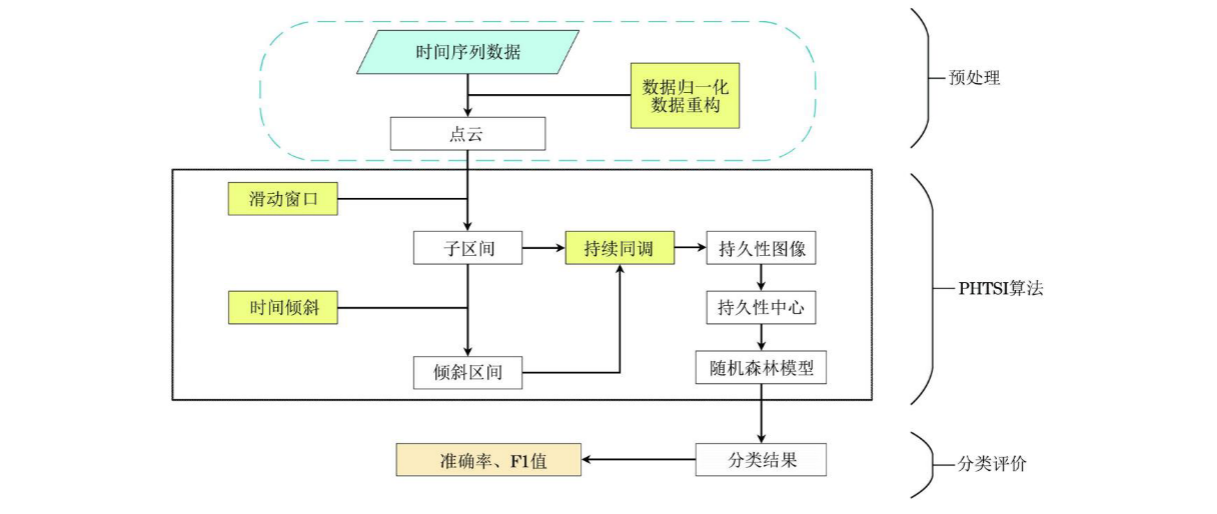
\includegraphics[width=1.0\textwidth]{figure/严银凯示意图.png}
    \caption{PHTSI算法示意图。}
    \label{fig:phtsi_algorithm}
\end{figure}

\paragraph*{步骤一:数据预处理}
在进行特征提取之前,原始时间序列数据需经过一系列预处理步骤,以确保数据的规范性并构建适用于拓扑分析的表示形式。首先需要做的是进行数据规范化,因为时间序列的数据通常的量纲不一致,通常会影响后续的分析过程,因此需要将数据尺度统一到特定区间。例如采用最小-最大规范化方法,将数据缩放到 $[0, 1]$ 的范围内。消除不同序列之间因为量纲差异可能导致的计算偏差问题。

随后需要将一维时间序列转化为二维的点云结构,在本章的开头就介绍了点云构造方法,对于原始时间序列中的每一个数据点 $a_t^i$,通过结合其后续点的差分信息,构造一个二维向量 $q_t^i = (a_t^i, a_{t+1}^i - a_t^i)$。这样的转换不仅保留了原始数据点的值,还融入了其局部变化趋势,初步揭示了序列的动态特性。
%
\paragraph*{步骤二:核心特征提取}
在构造完成点云之后,我们需要采用滑动窗口子序列划分方法,具体的做法是选择固定尺寸的滑动窗口及预设的滑动步长,将前一步构建的二维点云序列分割成若干个等长的子序列片段。这种局部化的处理方式有助于捕捉时间序列在不同阶段的局部模式,同时也能有效控制后续持久同调计算的复杂度。设窗口大小为 $w$ ,滑动步长为 $d_{step}$ (此处用 $d_{step}$ 以区别嵌入维度 $d$),则第 $i$ 个原始序列的第 $j$ 个子序列 $W_i^{j, 1}$ 可以表示为:
\begin{equation}
    W_i^{j, 1}=\left(q_{d_{step} \cdot j-d_{step}+1}^i, q_{d_{step} \cdot j-d_{step}+2}^i, \ldots, q_{d_{step} \cdot j-d_{step}+w}^i\right)
\end{equation}

接下来就是非常重要的时间序列倾斜方法,其目的是对子序列进行结构增强,用来揭示更丰富的时序依赖信息。“时间倾斜”是本研究中创新采用的一种策略,旨在通过对时间序列子区间内的点云施加与时间位置相关的加权,从而生成具有不同结构特性的新序列。
假设我们有一个从原始时间序列中提取的子区间(或称为滑动窗口内的点云),记为 $S$ 。该子区间由 $W$ 个按时间顺序排列的点组成:
\begin{equation}
    S=\left(p_1, p_2, \ldots, p_W\right)
\end{equation}
其中,$p_l$ 代表子区间内第 $l$ 个时间点对应的数据点(可能是一个向量,例如 $p_l=x\left(t_l\right)$ )。
时间倾斜方法通过将此子区间 $S$ 与两个不同的时间依赖函数 $f_1$ 和 $f_2$ 进行逐点乘法(或加权)来实现。

第一个倾斜变换采用线性函数 $f_1(k)=k$(其中 $k$ 为点在子序列中的序号,从1到 $w$ ),作用于子序列中的每个点 $q_k^{\prime}$(代表 $W_i^{j, 1}$ 中的第 $k$ 个点):
$$
    W_i^{j, 2}=\left(1 \cdot q_1^{\prime}, 2 \cdot q_2^{\prime}, \ldots, w \cdot q_w^{\prime}\right)
$$
此变换增强了子序列中后续点的影响。
第二个倾斜变换采用线性函数 $f_2(k)=w-k+1$ ,作用于子序列中的每个点 $q_k^{\prime}$ :
$$
    W_i^{j, 3}=\left(w \cdot q_1^{\prime},(w-1) \cdot q_2^{\prime}, \ldots, 1 \cdot q_w^{\prime}\right)
$$
此变换则增强了子序列中初始点的影响。
通过这种方式,原始子序列 $W_i^{j, 1}$ 及其两个倾斜版本 $W_i^{j, 2}$ 和 $W_i^{j, 3}$ 共同构成了后续拓扑分析的基础,使得算法能够从多个角度审视数据的内在结构。
到这里为止都是为了第四章的持续同调计算和持久性图生成做准备,后续具体内容会在第四章详细讲解。

\subsection{基于图的特征化时间序列表示} % 原3.5节
在标准的时间序列拓扑表示构建方法之外,为了更灵活地融入领域特定知识并优化持久同调的分析效果,Heo 与 Jung \cite{2} 近期提出了一种新颖的框架。该方法的核心在于引入了“特征化时间序列 (featured time series)”与“影响向量 (influence vector)”的概念,旨在通过调整时间序列的图表示来定制化持久同调的计算过程。

首先,一个特征化时间序列 $(\hat{T}, g)$ 由两部分构成:其一是特征增强的时间序列 $\hat{T}$,它将原始时间序列 $T$ 与一个特征组件 $T_f$ 配对,即 $\hat{T}(t) = (T(t), T_f(t))$。这里的特征组件 $T_f(t)$ 可以包含与单个时间点 $T(t)$ 相关的0阶特征(例如,某时刻的湿度状况)以及与相邻时间点对 $\{T(t_k), T(t_{k+1})\}$ 相关的1阶特征(例如,温度变化的幅度)。这些特征通常来源于特定领域的知识。其二是影响向量 $g$,它是一个非负实值函数,为每一个定义的特征(以及无特征状态)赋予一个“影响值”,用以量化该特征在后续分析中的重要性 。我们先引入一个存在异常区域的时间序列:
\begin{figure}[thbp!]
    \centering
    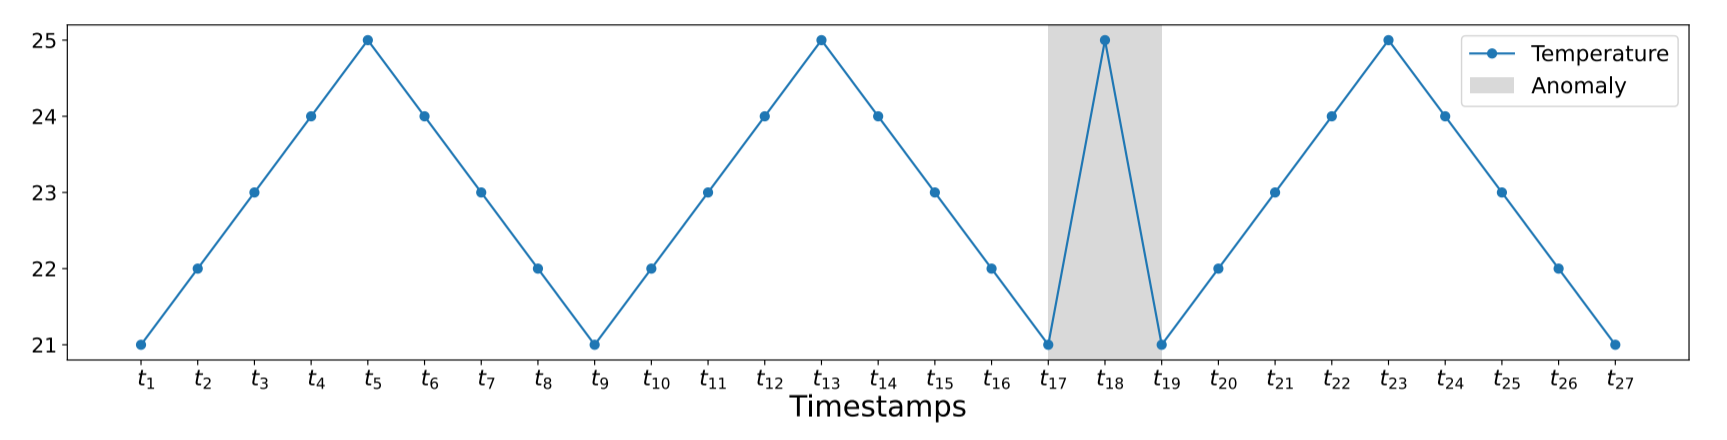
\includegraphics[width=1.0\textwidth]{figure/时间序列例子.png}
    \caption{存在异常的温度时间序列}
    \label{fig:phtsi_algorithm}
\end{figure}

该方法接着利用特征化时间序列 $(\hat{T}, g)$ 来构建一个加权图 $G=(V,E,\hat{W}_V,\hat{W}_E)$。其中,顶点集 $V$ 由时间序列中的观测值构成,边集 $E$ 通常连接连续的观测值。关键在于顶点权重函数 $\hat{W}_V$ 和边权重函数 $\hat{W}_E$ 的计算。它们并非简单地基于原始序列的频率,而是通过结合特征的出现次数和影响向量 $g$ 来确定。具体地,设 $F^0 = \{r_1, ..., r_m\}$ 为0阶特征集,$F^1 = \{s_1, ..., s_l\}$ 为1阶特征集。定义0阶计数矩阵 $C_0=(c_{ij}^0)$,其中 $c_{ij}^0$ 表示顶点 $v_i$ 与特征 $r_j$ (或无0阶特征状态 $\emptyset^0$) 在 $\hat{T}$ 中共同出现的次数。类似地,定义1阶计数矩阵 $C_1=(c_{ij}^1)$,其中 $c_{ij}^1$ 表示边 $e_i$ 与特征 $s_j$ (或无1阶特征状态 $\emptyset^1$) 在 $\hat{T}$ 中共同出现的次数。若影响向量 $g$ 对应0阶和1阶特征的分量分别为 $\vec{g_0} = (g(\emptyset^0), g(r_1), ..., g(r_m))$ 和 $\vec{g_1} = (g(\emptyset^1), g(s_1), ..., g(s_l))$,则顶点 $v_i$ 的权重和边 $e_i$ 的权重(也称为加权频率 $\hat{f}_{e_i}$)可以计算为:
\begin{equation}
    \hat{W}_V(v_i) = (C_0 \cdot \vec{g_0})_i
\end{equation}
\begin{equation}
    \hat{W}_E(e_i) = \hat{f}_{e_i} = (C_1 \cdot (\vec{g_1} + \vec{1}))_i
\end{equation}
其中 $\vec{1}$ 是全1向量,用于确保在 $\vec{g_1}=\vec{0}$ 时边权重与传统频率定义一致 。下面给出加权图的一个示例:
\begin{figure}[thbp!]
    \centering
    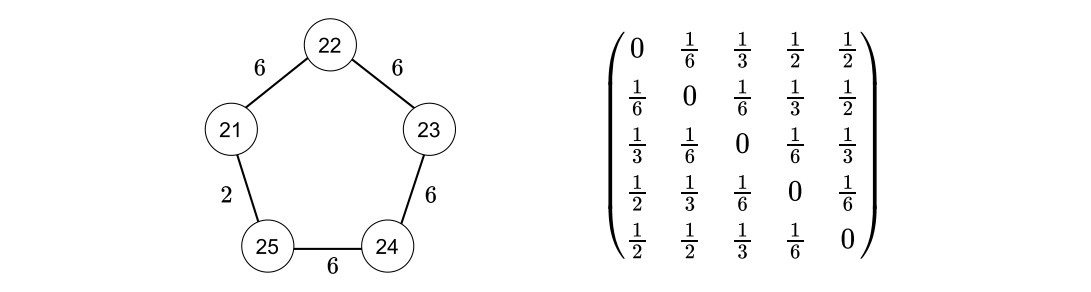
\includegraphics[width=1.0\textwidth]{figure/第三章加权图示意.png}
    \caption{时间序列的加权图与距离矩阵}
    \label{fig:phtsi_algorithm}
\end{figure}

随后,基于这个加权的图 $\hat{G}^g$,定义了节点间的距离度量 $\hat{d}$。对于图中的一条边 $e=\{a,b\}$,其长度 $L^g(e)$ 不仅考虑了其加权频率的倒数 $(\hat{W}_E(e))^{-1}$,还通过一个激活函数 $\rho$ (如 $\rho(z)=1-e^{-z^2}$ 对于 $z \ge 0$) 引入了与该边连接的两个顶点 $a,b$ 的加权频率 $\hat{W}_V(a)$ 和 $\hat{W}_V(b)$ 的影响:
\begin{equation}
    L^g(e) = (\hat{W}_E(e))^{-1} - \alpha (\rho(\hat{W}_V(a) + \hat{W}_V(b)))
\end{equation}
其中 $\alpha = \min_{e' \in E} (\hat{W}_E(e'))^{-1}$ 是一个归一化因子,确保边长非负。两个顶点 $v,w$ 之间的距离 $\hat{d}(v,w)$ 则定义为连接它们的最短路径上所有边长度 $L^g(e)$ 之和 。
\begin{equation}
    \hat{d}(v,w) = \min_{p: v \leadsto w} \left\{ \sum_{e \in p} L^g(e) \right\}
\end{equation}
这个经过特征和影响向量调整的距离度量 $(V, \hat{d})$ 构成了计算持久同调(例如通过Vietoris-Rips滤过)的基础。通过改变影响向量 $g$,研究者可以探索不同领域知识对时间序列拓扑结构的影响,具体构造方式如下图。Heo 与 Jung 最后证明了这种方法的一个重要性质:持久性图对于影响向量 $g$ 的变化是稳定的,即满足 $D_B(\text{dgm}_p(g), \text{dgm}_p(g')) \le C ||g-g'||_\infty$,其中 $D_B$ 是瓶颈距离,$C$ 是一个常数。这种稳定性保证了该增强方法在调整领域知识影响时的鲁棒性和结果的可靠性。
\clearpage
\begin{figure}[thbp!]
    \centering
    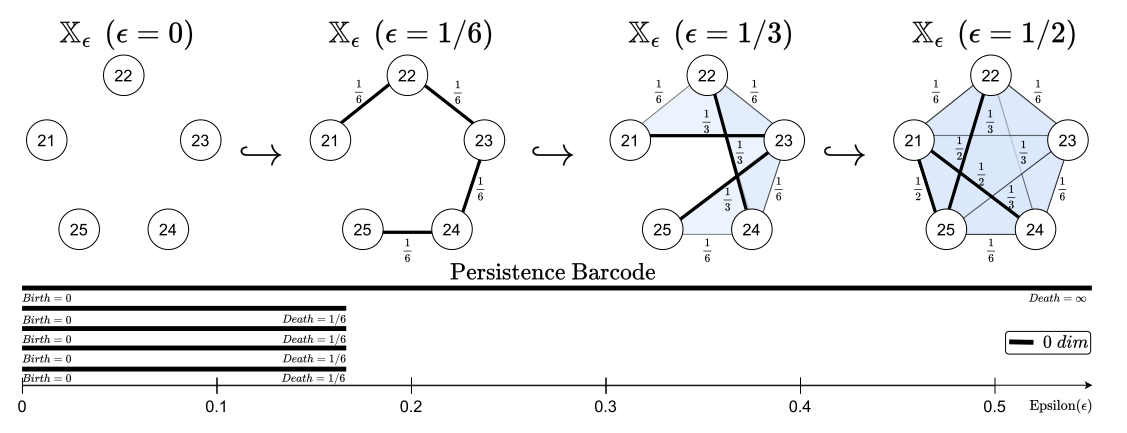
\includegraphics[width=0.8\textwidth]{figure/特征化时间序列.png}
    \caption{Rips过滤和条码图}
    \label{fig:phtsi_algorithm}
\end{figure}


之后我们通过一个表格来对比传统的点云嵌入方法与Heo \& Jung的特征化时间序列方法。表格中列出了两者在核心目标、距离度量来源、领域知识整合、调整机制、增强体现和理论稳定性等方面的主要区别。
\begin{table}[htbp]
    \centering
    \caption{传统点云嵌入与Heo \& Jung特征化时间序列方法的简明对比}
    \label{tab:embedding_comparison_concise_new}
    \begin{tabular}{>{\raggedright\arraybackslash}p{0.25\textwidth} >{\raggedright\arraybackslash}p{0.35\textwidth} >{\raggedright\arraybackslash}p{0.35\textwidth}}
        \toprule
        \textbf{比较维度}                          & \textbf{传统点云嵌入 (以TDE为例)} & \textbf{Heo \& Jung 的特征化方法} \\
        \midrule
        核心目标/输出                                &
        在欧几里得空间($\mathbb{R}^m$)中重构几何点云,代表系统状态。 &
        构建一个赋权图,并基于此定义一个可调整的度量空间 $(V, \hat{d})$ 作为拓扑分析输入。                                               \\
        \addlinespace
        距离度量来源                                 &
        通常是嵌入点之间的欧几里得距离。                       &
        基于图的边/点权重(由特征和影响向量决定)定义的最短路径距离 $\hat{d}(v,w)$。                                                  \\
        \addlinespace
        领域知识整合                                 &
        通常不直接在构造中融入,主要通过参数选择间接体现。              &
        通过“特征化时间序列”和“影响向量”显式、量化地融入距离度量的计算中。                                                             \\
        \addlinespace
        调整机制                                   &
        主要调整嵌入维度 $d$ 和时间延迟 $\tau$。             &
        主要调整“影响向量” $g$,改变特征对距离度量的影响。                                                                    \\
        \addlinespace
        “增强”体现                                 &
        优化参数以期更好地“展开”吸引子。                      &
        通过影响向量主动“调制”点间距离,使度量空间更能反映关注的结构。                                                                \\

        \bottomrule
    \end{tabular}
\end{table}

\subsection{时间序列的点云转换基础} % 新的小节,整合原3.2和3.3
上述特定方法以及其他多种基于点云的拓扑数据分析技术,其前提都是将原始的一维时间序列有效地转化为高维空间中的点云表示。状态空间重构为实现这一目标提供了核心的理论框架,其中时间延迟嵌入(TDE)是最为经典和基础的技术。本节将回顾这些基础方法及其相关的参数选择问题。

\subsubsection{状态空间重构概览} % 来自原3.2节的引言部分
我们需要将观测到的时间序列数据重构系统动力学状态空间,并构建其拓扑表示的方法.在许多科学和工程领域,我们面对的是复杂的动态系统,但往往只能观测到系统的一个或少数几个变量随着时间而变化,这种观测导致我们难以理解分析系统完整行为,所以我们需要从有限的,可能带有噪声的观测数据中,推断出驱动系统演化的潜在高维信息.传统的线性时间序列分析方法虽然在某些情况下有效,但往往难以捕捉复杂系统所固有的非线性特征和相互作用.状态空间重构是一个非常的好的解决办法,其基本思想是将低维的时间序列数据,通过特定的嵌入技术,转化为一个高维空间中的几何对象,这个重构出的状态空间在理想情况下能保持原始系统动力学的主要拓扑和几何特性.在众多状态空间重构技术中,时间延迟嵌入(TDE)扮演着基石性的角色.

\subsubsection{时间延迟嵌入 (TDE) 及其理论基础}
\paragraph{Takens 嵌入定理} % 原3.2.1节
TAKENS嵌入定理(Takens' Embedding Theorem)\cite{takens2006detecting}是由荷兰数学家Floris Takens在1981年提出的一个重要数学定理,主要应用于动力系统和时间序列分析领域。它提供了一种从单一标量时间序列数据中重构原始动力系统相空间的方法,尤其在研究混沌系统和非线性动力学时具有深远意义。

在介绍定理之前我们先来介绍两个基本概念:
\begin{itemize}
    \item \textbf{相空间(Phase Space)}: 动力系统的状态空间,描述系统所有可能状态的集合。对于一个n维动力系统,相空间是n维的。
    \item \textbf{吸引子(Attractor)}: 动力系统在长时间演化后趋向的状态或轨迹集合。吸引子可以是点、周期轨道或更复杂的结构,如奇异吸引子。
\end{itemize}
TAKENS嵌入定理的核心思想是,通过对时间序列进行适当的嵌入,可以在高维空间中重构出原始动力系统的相空间结构。具体来说,假设我们有一个一维时间序列$x(t)$,它是一个动力系统在时间上的投影。TAKENS定理指出,如果我们选择合适的\textbf{嵌入维度 $d$} 和\textbf{时间延迟 $\tau$},那么通过以下方式构造的 $d$ 维向量序列可以近似重构原始动力系统的相空间:
\begin{equation}
    \mathbf{x}_i = (x(t_i), x(t_{i+\tau}), x(t_{i+2\tau}), \ldots, x(t_{i+(d-1)\tau}))
\end{equation}
其中,$i$是时间序列的索引,$t_i$是时间点。

TAKENS定理的直观解释是:由于确定性动力系统中各个状态变量是相互耦合的,当前观测值及其过去(或未来)的延迟值序列中,蕴含了关于当前未被直接观测到的其他状态变量的信息.
补充: Sauer等人进一步完善了嵌入维度的条件,指出嵌入维度 $d$ 需要满足 $d \geq 2D_{sys}+1$, 其中 $D_{sys}$ 是原始动力系统吸引子的维数。这个定理的一个重要结论是,只要嵌入维度足够大,就可以通过重构的相空间来恢复原始系统的动力学行为,包括吸引子结构和混沌特性.

\paragraph{时间延迟嵌入 (TDE) 原理与实现} % 原3.2.2节
时间延迟嵌入(Time Delay Embedding, TDE) 是一种将一维时间序列数据转化为高维点云的技术,基于 Takens 嵌入定理。TDE 的基本思想是通过引入时间延迟和嵌入维度,将时间序列中的每个观测值与其过去的观测值组合成一个高维向量,从而重构出系统的相空间。这种方法能够捕捉到系统的非线性动力学特征,如周期性、混沌行为等。
TDE 的基本原理是将一维时间序列 \( s(t) \) 通过引入时间延迟 \( \tau \) 和嵌入维度 \( d \),转化为高维向量:
\begin{equation}
    \vec{x}(t) = \left[ s(t), s(t - \tau), s(t - 2\tau), \dots, s(t - (d - 1)\tau) \right]
\end{equation}
这些向量构成的集合形成了一个高维点云,即重构的相空间。根据Takens定理(及其后续改进),当嵌入维度 $d$ 足够大(例如 $d \geq 2D_{sys} + 1$,其中 $D_{sys}$ 为原始系统吸引子的维数)时,重构的相空间与原始系统的相空间在拓扑上是等价的。这种重构使得我们可以从单一观测变量中恢复系统的非线性动力学行为,例如吸引子结构或混沌特性。点云中的每个点代表系统在某时刻的状态,而点云的几何形状则反映了系统的长期演化规律。
%插入图片
\begin{figure}[thbp!]
    \centering
    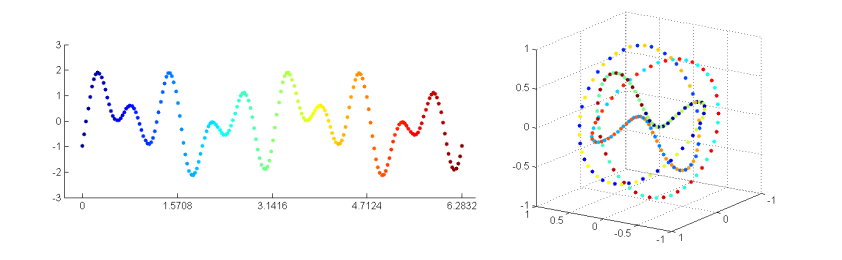
\includegraphics[width=1.0\textwidth]{figure/滑动窗口嵌入示意图、.png}
    \caption{周期性数据滑动窗口嵌入点云示意图}
    \label{fig:tde_example}
\end{figure}

\subsubsection{TDE 关键参数选择}
\paragraph{嵌入维度参数 $d$ 的选择} % 原3.2.3节
时间延迟嵌入(TDE)中嵌入维度 $d$ 的选择,直接决定了重构状态向量 $\vec{y}(t) = [x(t), \dots, x(t+(d-1)\tau)]$,对能否有效重构系统动力学至关重要。一个充分的 $d$ 值是保证重构空间能真实反映原始吸引子拓扑结构的基础。

若 $d$ 值选取 \textbf{过低},重构空间不足以完全“展开”高维吸引子,会导致原本分离的轨迹因投影而错误地靠近,产生所谓的 “伪近邻” (FNN)。这种拓扑结构的扭曲会严重影响后续基于重构空间的分析。

反之,若 $d$ 值选取 \textbf{过高},则会引入 “维度灾难” 问题。在有限数据下,高维空间的数据点变得稀疏,降低了依赖局部密度估计的分析方法(如关联维计算)的可靠性。同时,高维度也增加了计算负担并可能放大噪声。

因此,目标是找到最小的充分嵌入维度 $d_{min}$,它既能完全展开吸引子(消除FNN),又能避免不必要的高维问题。虽然Takens等理论给出了维度的理论下界(如 $d \ge 2D_{sys}+1$ 或 $d > 2D_A$, 其中 $D_A$ 为吸引子的某种维度度量),但通常需要根据数据进行估计。

实践中常用数据驱动方法估计 $d$。伪近邻法 (FNN)\cite{rhodes1997false}通过考察随着维度从当前值增加到 $d+1$(原文笔误,应为从一个维度 $d'$ 增加到 $d'+1$),近邻点对的距离是否显著增大来判断维度是否充分。当伪近邻比例降至阈值以下时,对应的 $d$ 可视为一个充分估计。Cao方法\cite{cao1997practical} 是对FNN的改进,通过分析统计量 $E1(d)$(邻近点距离的平均相对变化率)随 $d$ 的饱和行为来确定 $d$,并用 $E2(d)$ 辅助判断数据是否具有确定性。

总之,$d$ 的选择是一个需要在保证拓扑嵌入有效性与避免高维问题之间进行权衡的经验过程。通常需要结合使用多种估计方法,并考虑数据特性(长度、噪声)及分析目标。对估计值附近的 $d$ 进行敏感性分析,检验后续结果的稳定性,是验证选择合理性的常用手段。以下是一些常用的方法:

% --- End of LaTeX Snippet ---

\begin{table}[h!] % 使用 [h!] 尝试将表格放置在此处
    \centering % 表格居中
    \caption{时间延迟嵌入嵌入维度($d$)选择方法对比}
    \label{tab:embedding_dimension_methods_no_pros_cons_new}
    \begin{tabular}{
        >{\raggedright\arraybackslash}m{3cm} % 方法名称 (左对齐,自动换行)
        >{\raggedright\arraybackslash}m{4.5cm} % 核心原理 (左对齐,自动换行)
        >{\raggedright\arraybackslash}m{5cm}  % 原理阐释 (左对齐,自动换行)
        >{\raggedright\arraybackslash}m{4cm}  % 常用判据 (左对齐,自动换行)
        }
        \toprule % 顶部线条
        \textbf{方法名称}                        & \textbf{核心原理}             & \textbf{原理阐释}                                          & \textbf{常用判据/解释}                                                                       \\
        \midrule % 中间线条

        伪近邻法 (FNN) \cite{rhodes1997false}    & 邻近点在维度增加时的相对距离变化          & 维度不足时,投影导致假邻居;维度足够时,假邻居会散开,真邻居保持靠近                     & FNN随 $d$ 增加首次降至零或小阈值                                                                   \\
        \addlinespace % 增加行间距

        Cao方法\cite{cao1997practical}         & 近邻点对距离相对变化率的平均值 ($E1(d)$) & 旨在改进FNN,减少对阈值的依赖;观察变化率何时稳定                             & 绘制 $E1(d)$ 曲线,寻找其趋于平稳的 $d$ 值 。$E2(d)$ 用于区分确定性与随机性                                      \\
        \addlinespace

        符号动力学/熵方法\cite{matilla2021selection} & 符号序列的熵                    & 利用熵度量信息量或依赖性随参数的变化;将嵌入参数 $d, \tau$ 与最优时间窗口 $\tau_w$ 关联 & 寻找使熵最大化($\tau^*$)和最小化($\tau_w$)的延迟,通过 $\tau_w=(d-1)\tau^*$ (或类似形式)确定 $d$               \\
        \addlinespace

        Takens/Sauer 定理 (理论基础)               & 保证嵌入的微分同胚性                & 足够高的维度能“展开”吸引子,保持拓扑结构                                  & 理论要求 $d > 2D_{sys}$ (Takens改进后) 或 $d > 2D_A$ (Sauer),其中 $D_{sys}$ 为系统维数,$D_A$ 为吸引子某种维数 \\

        \bottomrule % 底部线条
    \end{tabular}
    \par % 确保表格后的文本在新行开始
    \vspace{0.5cm} % 在表格后增加一些垂直空间
\end{table}

下面我来介绍一下cao方法在论文中的运用:
曹亮月\cite{cao1997practical}提出的确定标量时间序列最小嵌入维数 $d_{min}$ 的方法,其核心思想是避免传统方法中主观参数的选择。该方法首先定义一个量 $a(i,d)$:
\begin{equation}
    a(i,d) = \frac{||y_i(d+1) - y_{n(i,d)}(d+1)||}{||y_i(d) - y_{n(i,d)}(d)||}
\end{equation}
其中 $y_i(d)$ 是 $d$ 维重构相空间中的点,$y_{n(i,d)}(d)$ 是其最近邻。然后计算 $a(i,d)$ 的均值 $E(d)$:
\begin{equation}
    E(d) = \frac{1}{N-d\tau}\sum_{i=1}^{N-d\tau} a(i,d)
\end{equation}
并考察其变化率 $E1(d)$:
\begin{equation}
    E1(d) = E(d+1)/E(d)
\end{equation}
当 $d$ 大于某个值 $d_0$ 后,$E1(d)$ 趋于饱和,此时 $d_0+1$ 即为最小嵌入维数。为区分确定性与随机信号,还引入了 $E^*(d)$:
\begin{equation}
    E^*(d) = \frac{1}{N-d\tau}\sum_{i=1}^{N-d\tau} |x_{i+d\tau} - x_{n(i,d)+d\tau}|
\end{equation}
及其变化率 $E2(d)$:
\begin{equation}
    E2(d) = E^*(d+1)/E^*(d)
\end{equation}
对于随机数据,$E2(d)$ 对所有 $d$ 均约等于1。下表总结了论文中部分实验结果:

\begin{table}[h!]
    \centering
    \caption{曹氏方法实验结果选例}
    \label{tab:cao_results_adjusted} % 建议修改label以区分
    % 请确保在导言区有 \usepackage{array}
    \begin{tabular}{|c|c|>{\centering\arraybackslash}p{3.5cm}|} % 删除了一列,并修改了对齐方式
        \hline
        \textbf{系统}                 & \textbf{Cao方法 $d_{min}$} & \textbf{与FNN对比}          \\
        \hline
        Hénon 吸引子                   & 2                        & 结果对数据长度不敏感               \\
        \hline
        Ikeda 吸引子                   & 4                        & 1000点时FNN结果不稳定           \\
        \hline
        Lorenz 吸引子                  & 3                        & 结果稳定                     \\
        \hline
        随机有色噪声                      & N/A ($E2 \approx 1$)     & FNN方法会误判为低维混沌            \\
        \hline
        Mackey-Glass ($\Delta=100$) & 17                       & FNN方法结果偏小 ($\sim$6)且依赖参数 \\
        \hline
        特定四维映射                      & 4                        & 1000点时FNN无法区分            \\
        \hline
        实验激光数据                      & 7                        & FNN结果在$d=7$后不稳定          \\
        \hline
    \end{tabular}
\end{table}

曹亮月通过对Hénon映射、Ikeda映射、Lorenz吸引子、随机有色噪声、高维Mackey-Glass方程、特定四维映射及真实激光数据等多种时间序列的实验验证了其方法的有效性。实验结果表明,该方法不仅能准确确定不同动力系统的最小嵌入维数 $d_{min}$,且对数据长度不敏感;尤为重要的是,它能有效区分确定性混沌与随机信号(如随机有色噪声,此时$E2(d) \approx 1$),并在处理高维系统(如Mackey-Glass)时显著优于传统的虚假最近邻(FNN)方法,后者在这些情况下常给出偏低或不稳定的结果且依赖于参数选择 。这些实验共同证明了曹氏方法在确定嵌入维数方面的鲁棒性、客观性和广泛适用性。

\paragraph{时间延迟参数 $\tau$ 的选择} % 原3.2.4节
在利用时间延迟嵌入技术重构复杂系统相空间的过程中,除了选择合适的嵌入维度 $d$ 之外,时间延迟参数 $\tau$ 的选取同样是\textbf{至关重要}的一环。它直接决定了构成嵌入向量 $\vec{y}(t) = [x(t), x(t-\tau), \dots, x(t-(d-1)\tau)]$ (此处统一符号,原文为 $x(t+\tau), \dots, x(t+(m-1)\tau)$)各分量之间的时间间隔。一个恰当的 $\tau$ 值是保证重构相空间能够有效“展开”原始动力系统吸引子,并保持其拓扑结构不变性的关键因素之一。

选择一个过小的 $\tau$ 值,会导致嵌入向量的相邻分量之间线性相关性过强,信息冗余度高。此时,$x(t)$ 与 $x(t-\tau)$ 非常接近,它们并未提供足够多的“新”信息来区分邻近的轨迹段。结果是,重构出的吸引子可能仍然是“折叠”或“挤压”在一起的,未能充分展现其在高维空间中的真实几何形态,这无疑会扭曲我们对系统动力学行为的理解。

相反,如果选择一个过大的 $\tau$ 值,虽然可以保证各分量之间的线性无关性甚至统计独立性,但 $x(t)$ 与 $x(t-(d-1)\tau)$ 之间可能已经失去了系统内在的动力学关联。这相当于在时间上跳跃得太远,使得嵌入向量无法捕捉到系统轨迹的连续演化特征和确定性结构,重构出的相空间可能变得杂乱无章,甚至接近随机噪声的表现,同样无法真实反映原始动力学。

因此,$\tau$ 的选择面临着一个\textbf{核心的权衡}:既要足够大以确保嵌入向量的各分量包含足够独立的信息,从而有效展开吸引子;又要足够小以保留系统随时间演化的内在关联性与动力学规律。一个不恰当的 $\tau$ 值将直接影响后续所有基于重构相空间的分析,包括分形维数的计算、Lyapunov 指数的估计、系统的预测精度以及噪声抑制的效果等。鉴于其对整个相空间重构质量和后续分析有效性的\textbf{决定性影响},如何合理地选择时间延迟 $\tau$ 成为了时间序列非线性分析中的一个基本且关键的问题。下面将展示几种常用的 $\tau$ 值选择策略及其背后的原理。

\begin{table}[h!]
    \centering
    \caption{时间延迟嵌入时间延迟 ($\tau$) 选择方法对比}
    \label{tab:time_delay_tau_methods_compare_new}
    \begin{tabular}{
        >{\raggedright\arraybackslash}m{3cm}
        >{\raggedright\arraybackslash}m{4.5cm}
        >{\raggedright\arraybackslash}m{5cm}
        >{\raggedright\arraybackslash}m{4cm}
        }
        \toprule
        \textbf{方法名称}                              & \textbf{核心原理} (分析的度量)                 & \textbf{原理阐释} (为何有效)                        & \textbf{常用判据/解释}                                                                \\
        \midrule

        自相关函数 (ACF)\cite{kantz2003nonlinear}       & 时间序列与其滞后版本间的线性相关性                     & 寻找 $x(t)$ 与 $x(t+\tau)$ 线性无关的最小延迟           & $\tau$ 取 ACF 首次降至零 或首次降至 $1/e \approx 0.37$ 的值                                  \\
        \addlinespace

        平均互信息 (AMI)\cite{wallot2018calculation}    & $x(t)$ 与 $x(t+\tau)$ 之间的统计依赖性 (信息论度量) & 寻找 $x(t)$ 与 $x(t+\tau)$ 共享信息量最少的延迟,以捕捉非线性结构 & $\tau$ 取 AMI 函数 $I(\tau)$ 的第一个局部最小值                                             \\
        \addlinespace

        C-C 方法 (基于关联积分)\cite{cai2008determination} & 分析关联积分在不同 $\tau, d$ 下随邻域半径 $r$ 的变化    & 通过检验不同时间窗内数据的统计独立性与几何展开程度寻找最优参数             & 寻找特定统计量(如 $\Delta \bar{S}_2(t)$ 或 $\sigma_{cor}(t)$)首次穿零或达极小值对应的 $t$ (即 $\tau$) \\
        \addlinespace

        几何/直观方法                                    & 观察时间序列图或相图的特征时间尺度                     & 基于对系统动力学行为的先验知识或直观观察估计                      & $\tau$ 常取为主要周期或特征时间的某个分数(如 1/4 到 1/10)                                          \\
        \bottomrule
    \end{tabular}
    \par
    \vspace{0.5cm}
    \textit{注意:选择 $\tau$ 与选择 $d$ 密切相关。实际应用中 $\tau$ 的选择常带有启发性,需测试不同值的影响。AMI 通常被认为是较优选择。}
\end{table}

\textbf{相关实验}: Wallot 和 Mønster(2018)\cite{wallot2018calculation} 该实验选择时间嵌入参数时,首先使用平均互信息(AMI)确定延迟参数 $\tau$。对于一维时间序列 $x(t)$,AMI 的计算公式为
$$I(x(t),x(t+\tau))=\sum_{i,j}p_{ij}(\tau)\log\left(\frac{p_{ij}(\tau)}{p_{i}p_{j}}\right)$$
其中 $p_i$ 是数据点在直方图第 $i$ 个bin的概率,$p_{ij}(\tau)$ 是 $x(t)$ 在 bin $i$ 且 $x(t+\tau)$ 在 bin $j$ 的联合概率。对于 $d_{orig}$ 维时间序列(此处用 $d_{orig}$ 表示原始信号的维度,以区别嵌入维度 $d$),采用各维度 AMI 的平均值。选择 $\tau$ 的依据是 $I(\tau)$ 的第一个局部最小值或其值首次低于某个阈值(例如 $1/e$)。确定 $\tau$ 后,使用虚假最近邻(FNN)方法选择嵌入维度 $d$。对于 $d_{orig}$ 维时间序列 $x_j(t)$,在由 $d$ 个延迟副本(总维度为 $d \times d_{orig}$)构成的相空间中,点 $y(t)$ 与其第 $r$ 个最近邻 $y^{(r)}(t)$ 的欧氏距离平方为
$$R_{d,d_{orig}}^{2}(t,r)=\sum_{j=1}^{d_{orig}}\sum_{k=0}^{d-1}[x_{j}(t-k\tau)-x_{j}^{(r)}(t-k\tau)]^{2}$$
当增加一个延迟副本到 $d+1$ 时,新的距离平方为
$$R_{(d+1),d_{orig}}^{2}(t,r)=R_{d,d_{orig}}^{2}(t,r)+\sum_{j=1}^{d_{orig}}[x_{j}(t-d\tau)-x_{j}^{(r)}(t-d\tau)]^{2}$$
如果从 $d \times d_{orig}$ 维到 $(d+1) \times d_{orig}$ 维时,邻居间的距离发生显著变化(依据阈值 $R_{tol}$ 和 $A_{tol}$ 判断),则该邻居为虚假最近邻。选择使FNN百分比降至接近零的最小 $d$ 值。

\paragraph{嵌入参数选择的综合考量} % 原3.2.4节末尾的总结
嵌入维度 $d$ 的选择旨在确保重构空间具有足够的维度,以完全“展开”动力系统的吸引子,避免因维度不足导致的轨迹交叉和结构误判(即伪近邻现象)。我们探讨了多种估计最小充分嵌入维度的方法,包括基于几何直观的伪近邻法 (FNN) 及其改进(如 Cao 方法),以及基于系统理论的 Takens/Sauer 定理等。FNN 及其变种通过考察邻近点在维度增加时的相对距离变化来寻找合适的 $d$,而理论定理则提供了嵌入有效性的数学保证,但其给出的往往是维度的上限而非最优实用值。

时间延迟 $\tau$ 的选择则关注于如何设置嵌入向量中各分量之间的时间间隔,以在保证分量间足够统计独立性(从而有效利用 $d$ 维空间)与保留系统时间演化内在关联性之间取得平衡。$\tau$ 过小导致信息冗余,$\tau$ 过大则可能丢失动力学信息。常用的 $\tau$ 选择方法包括分析时间序列自相关性(如自相关函数 ACF 法,主要关注线性相关)和信息论依赖性(如平均互信息 AMI 法,能更好地处理非线性相关),以及一些试图结合几何特性或同时考虑 $d$ 和 $\tau$ 的方法(如 C-C 方法)。其中,AMI 方法因其对非线性动力学的适应性而被广泛推荐。

值得强调的是,$d$ 和 $\tau$ 的选择并非完全独立的过程。它们共同定义了重构所利用的时间跨度,即所谓的“时间窗口” $\tau_w = (d-1)\tau$ 。某些方法(如 C-C 方法)正是着眼于这个时间窗口的优化。更重要的是,实际应用中参数的选择往往带有启发性,不存在一个适用于所有类型时间序列(如长/短、含噪/纯净、周期/混沌)的通用“万能”方法。

因此,在实践中,研究者通常不会仅仅依赖单一方法的建议值,而是倾向于尝试应用多种不同的方法(例如结合几何类、信息论类等手段)来估计 $d$ 和 $\tau$,并对结果进行相互比较和验证。同时,必须充分考虑所分析时间序列的具体特性,例如其采样频率、噪声水平以及内在的特征时间尺度等,这些因素都可能影响不同选择方法的表现和适用性。进行参数敏感性分析也极为关键:考察在一个根据初步方法确定的合理 $d$ 和 $\tau$ 参数值邻域内,后续计算得到的动力学不变量(如关联维、Lyapunov指数)或模型的预测误差是否保持稳定,是验证参数选择鲁棒性的重要手段。最终的选择决策,应当是在综合考量多种方法建议、数据自身特点、参数敏感性测试结果以及具体科学研究目标的基础上作出的。

总而言之,只有通过这样细致、多角度的比较、选择和验证过程,才能更有信心地确保所构建的重构相空间是原始动力系统的一个有效且可靠的拓扑等价表示,从而为后续深入的非线性动力学分析和应用奠定坚实的基础。

\subsubsection{其他替代性嵌入技术} % 原3.3节
\paragraph{} % 引言段落
基于嵌入理论的非线性动力系统分析已广泛应用于时间序列的建模、预测、信号检测与分类。其核心思想是通过嵌入过程从单变量时间序列重构高维状态空间,以揭示系统潜在的动力学特性。Takens嵌入定理为标准的时间延迟嵌入(Time-Delay Embedding, TDE)提供了坚实的理论基础,该方法通过使用信号的延迟副本构建状态向量。

然而,标准的TDE方法在处理真实世界的复杂数据时面临显著挑战。Takens定理的理想化假设(如无限长、无噪声数据)往往难以满足,使得TDE的效果高度依赖于嵌入维数 $d$ 和时间延迟 $\tau$ 的精确选择——而这通常缺乏统一标准,且对结果影响巨大。此外,单一的均匀延迟 $\tau$ 可能无法有效捕捉具有多个内在时间尺度的复杂系统动力学。

正是这些局限性,尤其是标准TDE在参数选择上的困难以及对多尺度动态捕捉能力的不足,极大地激发了研究者们探索和发展替代性嵌入技术的热情。 这些替代方法旨在从不同角度克服TDE的缺点,例如通过引入导数信息来补充状态描述,利用主成分分析(PCA)优化嵌入维度和方向,采用多变量嵌入整合来自多个传感器或来源的信息,或设计非均匀嵌入以更好地适应变化的或多重的时间尺度。这些技术共同构成了一个更加丰富的嵌入方法工具箱,为从观测数据重构和理解复杂系统动力学提供了更多样化且可能更鲁棒的途径。接下来,我们将介绍其中几种重要的替代嵌入方法。

\paragraph{值-差分嵌入} % 原3.3.1节
一种直观的替代思路体现在严银凯等人(2024)针对时间序列分类任务所采用的方法中。他们并未采用高维的TDE,而是选择将原始的单变量时间序列 $\{a_t\}$ 直接映射到一个二维的点云空间。具体地,该方法构建的二维点集 $\{q_t\}$ 中,每一个点 $q_t$ 的坐标由该时刻的观测值 $a_t$ 以及它与下一时刻观测值的一阶差分 $a_{t+1}-a_t$ 构成,即 $q_t = (a_t, a_{t+1}-a_t)$。根据作者的阐述,这种特定的二维构造旨在使生成的点云能够同时反映时间序列的当前状态(由值 $a_t$ 体现)和其短期的变化趋势(由差分 $a_{t+1}-a_t$ 近似),从而捕捉所谓的“周期上和周期内的特征”。

相较于需要仔细调参的标准TDE,这种固定的二维嵌入方式显著简化了嵌入过程,避免了复杂的参数搜索。它为后续应用拓扑数据分析(如持续同调)提供了一种直接的、蕴含了原始值与变化率信息的低维输入表示。尽管这种特定的低维嵌入可能不像满足Takens定理条件的高维TDE那样,能够保证在拓扑意义下完全重构原始动力系统的吸引子,但它代表了在特定研究背景下,为了处理特定问题(如简化流程、突出变化信息)而对嵌入策略进行的适应性构造与尝试。这类方法与其他替代嵌入技术,如导数嵌入、主成分分析嵌入等,共同丰富了从时间序列数据中提取动力学或结构特征的工具箱。

\paragraph{导数嵌入} % 原3.3.2节
作为时间延迟嵌入(Time-Delay Embedding, TDE)的一种替代性状态空间重构技术,导数嵌入\cite{lekscha2018phase}(Derivative Embedding)利用信号的(近似)连续导数来构建嵌入向量。例如,一个包含位置、速度和加速度信息的三维导数嵌入向量可以表示为 $(x(t), \frac{dx}{dt}, \frac{d^2x}{dt^2})$。其核心思想在于,动力系统的状态不仅取决于其当前位置 $x(t)$,也与其变化率(如速度 $\frac{dx}{dt}$、加速度 $\frac{d^2x}{dt^2}$ 等)密切相关。通过将这些导数信息纳入嵌入向量,可以在重构的状态空间中直接捕捉系统的动态变化特性。从理论视角看,导数嵌入可被视为一种基于系统底层微分方程表示来重构其相空间的方法。若一个物理系统能由一组微分方程精确描述,则系统的状态变量及其各阶导数构成了描述该系统演化的自然坐标系。因此,当研究者认为所观测时间序列源自一个由微分方程控制的潜在系统时,导数嵌入提供了一种直观且可能更自然的动力学展开方式,它将分析的焦点从系统的“状态”(由延迟值表示)转移到了系统的“变化”(由导数值表示),为理解那些变化率本身包含关键信息的系统动力学提供了重要的补充视角。

为适应不同的应用需求,导数嵌入的基本概念已被进一步扩展并常与其他技术结合,催生出功能更强大的变体。其中一个重要的变体是导数延迟嵌入(Derivative Delay Embedding, DDE),它被特别设计用于增量式地将时间序列数据转换到嵌入空间,尤其适用于在线流式数据的处理场景。DDE的一个关键优势在于其能够在不依赖于固定窗口长度或数据良好对齐假设的情况下,有效保留数据的内在递归模式,同时保持较高的计算效率,使其非常适合实时捕捉时变特性并进行在线建模与分类任务。另一个值得注意的框架是延迟微分分析(Delay Differential Analysis, DDA),它通常结合了导数信息与非均匀的时间延迟信息,形成所谓的“函数嵌入”(functional embeddings)。通过整合来自不同时间尺度的延迟值和导数值,DDA旨在更全面地刻画复杂系统的动力学特征,能够应用于更广泛的问题,包括处理长度较短或含有缺失值的稀疏时间序列数据。这些变体的出现,例如常与非参数马尔可夫地理模型(MGM)结合构成DDE-MGM方案,反映了导数嵌入的实用价值往往在与其他技术集成时得到显著放大,从而形成更全面的分析框架。

延迟微分方程 (DDEs) \cite{lainscsek2015delay}是时间序列分析中的一种有力工具,它通过函数嵌入巧妙地结合了导数嵌入与非均匀延迟嵌入的思想。一个基础的线性DDE可以表示为:
\begin{equation}
    \dot{x}(t) = a x(t-\tau)
\end{equation}
其中 $\dot{x}(t)$ 代表信号 $x(t)$ 的时间导数,$x(t-\tau)$ 是信号在过去某一时刻 $t-\tau$ 的值,而 $a$ 和 $\tau$ 分别是系数和时间延迟。这类方程能够揭示信号的频率特性,例如对于谐波信号 $x(t) = A\cos(\omega t + \phi)$,其延迟 $\tau$ 与频率 $\omega$ 存在特定关系,如 $\tau = \frac{(2n-1)\pi}{2\omega}$,且系数 $a = (-1)^n\omega$。DDEs的分析不止于线性范畴,例如非线性DDE,如下式所示:
\begin{equation}
    \dot{x}(t) = a x(t-\tau)^2
\end{equation}
则可以用于检测信号中的非线性相互作用,例如二次相位耦合。更一般地,DDEs可以包含线性和非线性项的组合,例如:
\begin{equation}
    \dot{x}(t) = a_1 x(t-\tau) + a_2 x(t-\tau)^2
\end{equation}
其中非线性项的系数(如 $a_2$)的存在与否能够指示特定非线性现象(如二次频率耦合)的出现。通过构建和分析这些基于时间序列数据选取的DDE模型,可以有效地揭示和分类复杂系统的动态行为。

导数嵌入及其相关概念已在多个领域得到应用。在流式数据分析方面,DDE-MGM方案已被成功用于时间序列的在线建模与分类,据报道在保持高效率的同时取得了先进的性能。生物医学信号处理是另一个重要的应用领域,例如DDA已被用于区分心电图(EKG)数据反映的不同心脏状况,以及区分帕金森病患者与健康对照组的脑电图(EEG)数据。更一般地,导数嵌入可服务于时间序列的信号检测与分类任务。如前所述,DDA等方法还可用于时域内的谱分析,包括频率分析、耦合检测和双谱估计。在金融领域,虽然不直接称为导数嵌入,但相关的随机微分方程(SDEs)是建模资产价格等随机过程的核心工具,对于金融衍生品定价至关重要,其理论基础与导数概念紧密相连。此外,在变化检测领域,许多时间序列变化检测算法是遥感(如利用Landsat时间序列监测地表覆盖变化)和生物监测等应用中的关键组成部分,这些算法有时也隐式或显式地利用了序列的变化率信息。

\paragraph{主成分分析嵌入} % 原3.3.3节
主成分分析(Principal Component Analysis, PCA)\cite{broomhead1986extracting}是一种经典的线性降维技术,其核心思想是通过正交线性变换将原始高维数据投影到一个新的低维坐标系中,旨在降维的同时尽可能多地保留由方差衡量的原始数据信息。这个新坐标系的轴被称为主成分(Principal Components, PCs),它们相互正交且按照其捕捉到的原始数据方差大小进行排序:第一主成分(PC1)对应数据方差最大的方向,第二主成分(PC2)是在与PC1正交的子空间中方差次大的方向,以此类推。本质上,PCA是在寻找数据变异性最大的方向。

PCA的计算过程通常涉及几个关键步骤。首先,对原始数据的各个特征进行标准化处理,使其具有零均值和单位方差,以消除不同特征尺度差异可能带来的影响。其次,计算标准化后数据特征之间的协方差矩阵,该矩阵反映了特征间的线性相关性。接着,对协方差矩阵进行特征值分解,求解特征向量方程 $AX=\lambda X$(其中 $A$ 是协方差矩阵,$X$ 是特征向量,$\lambda$ 是对应的特征值)。特征向量指明了主成分的方向,而特征值的大小则量化了该主成分所解释的方差。通过将特征值从大到小排序,选择前 $k$ 个最大特征值对应的特征向量,便构成了最优的 $k$ 维投影子空间。最后,将原始标准化数据投影到这个由选定 $k$ 个特征向量张成的子空间上,即可得到降维后的数据表示。

这种将高维数据映射到由主要主成分构成的低维空间的过程,其本身就是一种数据嵌入(Embedding)的方法\cite{gibson1992analytic}。这个低维表示试图在更紧凑的空间中保留原始数据的核心结构(以方差最大化为目标)。作为一种无监督的降维技术,PCA在机器学习流程中扮演着重要角色,常被用作预处理步骤,特别是在处理具有极高维度特征的数据时(例如文本分析中的词袋模型、图像数据或基因表达数据)。通过PCA降低维度,可以简化数据表示,减少计算负担,去除部分噪声,并可能提高后续机器学习算法(如分类器、聚类算法)的训练效率和性能。此外,PCA也是探索性数据分析的有力工具,通过将数据投影到二维或三维空间进行可视化,有助于直观理解数据的内在结构、聚类趋势和分布特征。例如,在多变量时间序列(MTS)分析中,可以对表示为矩阵的MTS数据应用PCA,并利用其主成分和特征值来定义MTS之间的相似性度量。

作为一种基础且广泛应用的嵌入与降维技术,PCA具有显著的优点。其计算相对高效,并且作为一种确定性算法,对于给定的数据集每次运行结果都相同。PCA擅长保留数据的全局结构和最大化方差,并且由于其线性变换的本质,其过程和结果相对透明,易于理解和解释(主成分可视为原始特征的线性组合)。同时,PCA也可有效用于数据压缩和降噪。然而,PCA也存在一些固有的局限性。最主要的是其线性假设,使得它可能无法有效捕捉数据中复杂的非线性模式和流形结构。其次,PCA以最大化方差为目标,但这并不总能保证保留对特定下游任务(如分类)最重要的判别信息,例如可能无法很好地区分本身方差不大但类别边界清晰的簇,也可能不如某些方法(如LLE, t-SNE)那样能有效保持数据的局部邻域结构。此外,PCA对原始特征的尺度非常敏感,因此通常需要进行数据标准化预处理。主成分必须相互正交的约束在某些情况下也可能是一种限制。同时,PCA对数据中的离群点也比较敏感。在某些特定领域(如遗传学中表示复杂的混合血统结构),PCA可能不如某些非线性方法或专门设计的模型有效,尽管后者可能面临解释性更差的问题。

\paragraph{多变量嵌入} % 原3.3.4节
许多现实世界的复杂系统,如气候系统、金融市场、生物过程或工业流程,其行为本质上是由多个相互作用的变量共同决定的,其观测数据通常以多变量时间序列(Multivariate Time Series, MTS)的形式出现。传统的单变量嵌入方法,即独立地对每个变量(通道)进行时间延迟嵌入等操作,常常忽略了变量之间可能存在的关键交叉相关性、耦合关系和因果影响。多变量嵌入(Multivariate Embedding)技术\cite{barnard2001embedding}的核心动机正是为了克服这一局限,旨在通过同时利用来自所有或部分相关观测变量的信息来重构系统的状态空间,从而更准确地捕捉和保留这些变量间的相互依赖性。理解这种相互作用对于建模耦合系统的动力学、预测其未来行为以及揭示其内部的因果网络结构至关重要。因此,对于需要理解系统层面交互而非孤立信号行为的应用,多变量嵌入是从单变量分析向系统整体分析的必要演进。

实现多变量嵌入存在多种途径,它们通常是对单变量方法的扩展或与其他技术的结合。最直接的扩展是均匀多变量嵌入,它简单地将每个变量的标准延迟嵌入向量连接(concatenate)起来,形成一个更高维度的联合状态向量。例如,对于 $p$ 个变量,若每个变量 $i$ 使用嵌入维数 $d_i$ 和延迟 $\tau_i$,则总嵌入维数为 $d_{total} = \sum_{i=1}^{p} d_i$。然而,考虑到不同变量或同一变量的不同历史时刻可能对当前状态有不同程度或不同时间尺度的影响,非均匀多变量嵌入(有时也称为混合嵌入)被提出。这类方法试图从所有变量的可能延迟组合中,通过复杂的模型选择或优化过程,识别出一个最优的、通常更紧凑的混合延迟向量,以更有效地解释目标变量或重构系统状态。除了基于延迟嵌入的扩展,其他技术也被纳入多变量嵌入的范畴。例如,主成分分析(PCA)可以应用于视为矩阵的MTS数据,其提取的主成分和特征值可用于定义MTS之间的相似性度量。针对MTS的结构复杂性分析,则可以采用基于熵的方法,如结合多元经验模态分解(Multivariate Empirical Mode Decomposition, MEMD\cite{rehman2010multivariate})的多元样本熵(Multivariate Sample Entropy, MSE),该方法能同时考虑通道内和通道间的复杂性。特别地,多变量嵌入向量构成了许多现代因果推断方法的基础,例如多元格兰杰因果(Granger Causality)检验和传递熵(Transfer Entropy)及其条件化或部分化的变体(如Partial Transfer Entropy, PTE)。这些方法利用嵌入向量来量化一个变量的过去对另一个变量未来的预测能力(同时可能控制其他变量的影响),其中嵌入向量的构建方式(如维数 $d$ 和延迟 $\tau$ 的选择)对因果分析结果的准确性具有显著影响。

多变量嵌入的主要优势在于能够提供一个更全面的系统视图。通过整合多个变量的信息,它能够捕捉单变量分析可能忽略的变量间相互作用,从而可能在非线性系统检测、时间序列预测等任务中产生比单变量方法更鲁棒和准确的结果。此外,对于理解耦合系统中的因果关系、信息流向和网络拓扑结构,多变量嵌入更是不可或缺的基础。然而,多变量嵌入也带来了新的、显著的挑战。最突出的是“维度灾难”(Curse of Dimensionality)问题:同时考虑多个变量及其各自的延迟会急剧增加嵌入空间的维度 $d$。这不仅使得状态空间变得稀疏,影响基于近邻的估计(如熵、互信息)的准确性和鲁棒性,也使得参数选择变得异常复杂。无论是为每个变量确定合适的 $d_i, \tau_i$(均匀嵌入),还是在巨大的组合空间中搜索最优的混合延迟向量(非均匀嵌入),都极具挑战性。随之而来的是计算成本的显著增加,包括参数搜索和处理高维数据的开销。此外,为了获得可靠的统计估计,多变量嵌入通常需要更长的时间序列数据来充分“填充”高维状态空间,并且需要有效处理多变量数据特有的问题,例如不同通道可能存在的非平稳性(可能需要MEMD等自适应预处理技术)。如何有效管理这种因变量和参数组合爆炸性增长带来的复杂性,是多变量嵌入研究的核心挑战之一,这也推动了对高效且信息丰富的变量/延迟选择策略(常借鉴非均匀嵌入思想)的研究,旨在使多变量嵌入在实践中更加可行和有效。

\paragraph{非均匀嵌入} % 原3.3.5节
标准的时间延迟嵌入(Time-Delay Embedding, TDE)通过采用一个固定的、均匀的时间延迟 $\tau$ 来构建状态向量,其形式通常为 $[x(t), x(t-\tau), x(t-2\tau), \dots]$。然而,许多自然和工程系统展现出跨越多个时间尺度的复杂动力学行为,例如可能同时存在快速振荡和缓慢漂移。使用单一固定的 $\tau$ 值可能无法同时有效捕捉这些不同尺度的特征:较小的 $\tau$ 可能适合解析快速动态,但会使慢动态在嵌入空间中显得拥挤;反之,较大的 $\tau$ 可能适合展开慢动态,但会丢失快速动态的细节信息。非均匀嵌入(Non-uniform Embedding, NUE)\cite{jia2019detecting}正是为了解决标准TDE的这一局限性而提出的。它允许在嵌入向量中使用一组不同的、非均匀的时间延迟 $(\tau_1, \tau_2, \dots, \tau_{d-1})$ 来构建 $d$ 维状态向量,例如形式可以是 $[x(t), x(t-\tau_1), x(t-\tau_1-\tau_2), \dots]$,或者更一般地使用相对于当前时间 $t$ 的一组绝对延迟 $\{\tau'_1, \tau'_2, \dots, \tau'_{d-1}\}$ 构成嵌入向量 $[x(t), x(t-\tau'_1), x(t-\tau'_2), \dots]$。NUE的核心思想在于摆脱选择单一 $\tau$ 的任意性和潜在信息冗余,通过数据驱动或基于特定准则选择一组最能反映系统动力学本质的延迟,构建一个可能维度更低、信息更丰富的状态空间表示,从而更好地适应真实世界系统的复杂性和多尺度特性。

非均匀嵌入不仅可以应用于单变量时间序列,还可以自然地扩展到多变量场景,此时通常称为混合嵌入(Mixed Embedding),即从所有可用变量的不同时间延迟中选择一个最优的组合来构成联合嵌入向量。此外,NUE还可以与导数嵌入等技术结合使用,例如在延迟微分分析(Delay Differential Analysis, DDA)框架中。然而,尽管NUE在概念上更具灵活性和适应性,其实施面临的主要挑战在于如何有效地确定最优的非均匀延迟集合。可能的延迟组合数量随着嵌入维数 $d$ 和考虑的最大延迟 $L$ 呈指数级增长,使得穷举搜索在实践中通常不可行。因此,如何高效地搜索并评估候选延迟组合成为NUE研究的核心问题。

为了应对延迟选择的挑战,研究者们提出了多种基于特定评估准则和搜索策略的方法。许多方法依赖于迭代选择过程,如贪婪前向选择(greedy forward selection),在每一步选择能最大程度改进某个预定义准则(如预测精度、互信息减少量等)的下一个延迟。然而,贪婪策略容易陷入局部最优解。另一个关键挑战在于评估准则本身的计算,尤其是在高维空间中。许多先进的NUE方法采用信息论度量,如条件互信息(Conditional Mutual Information, CMI)\cite{jia2020refined},来评估候选延迟的相对重要性或对目标变量的解释力。但是,CMI的准确估计在高维空间中非常困难,易受“维度灾难”问题的影响,导致基于数据密度的估计(如基于直方图或核密度估计)变得不可靠。

为克服这些困难,研究界发展了多种先进技术。在信息论方法方面,提出了基于混合嵌入的条件互信息(MIME)及其多元扩展(Partial MIME, PMIME)等框架,它们通常结合高效的熵估计器(如k-近邻(kNN)估计器)以提高在高维空间中的估计稳定性和效率,旨在优化嵌入向量并绕过传统参数($d$, $\tau$)选择的困境。为缓解CMI估计中的维度问题,有研究提出使用低维近似(Low-dimensional Approximation, LA)方法,用一系列低维CMI项的和来近似高维CMI。在搜索策略方面,除了贪婪选择,还探索了混合搜索策略(如结合前向选择与后向剔除)或采用启发式全局优化算法(如二进制粒子群优化, BPSO)直接在延迟组合空间中搜索,以期找到比贪婪搜索更优的解并移除冗余信息。此外,还有基于重构吸引子几何特性(如最大化其展开程度)的确定性方法,以及利用拓扑数据分析工具(如持续同调)来识别时间序列中具有动力学意义时间尺度的方法,例如SToPS(Significant Times on Persistent Strands)通过分析持续同调图谱构建特征时间谱来指导非均匀延迟的选择。这些方法的涌现反映了NUE领域正致力于开发实用且鲁棒的延迟选择方法论。

相较于均匀嵌入,非均匀嵌入具有显著的潜在优势。它能够更好地适应和表示具有多个内在时间尺度的复杂系统动力学,可能在时间序列预测、耦合检测等任务中提供更优的状态空间重构,进而带来性能提升。同时,它避免了选择单一固定延迟 $\tau$ 的主观性和困难,并通过只选择最相关的延迟可能产生维度更低、更简洁的嵌入向量,减少信息冗余。先进的NUE方法(如PMIME)还能有效检测多元系统中的直接耦合。然而,NUE的主要缺点在于确定最优延迟集合的过程非常复杂且计算成本高昂,尤其对于高维系统或采用全局优化策略时。此外,若未使用有效的缓解技术,在高维空间中准确估计信息论准则(如CMI)仍然是一个挑战,并且某些NUE选择方法的动力学可解释性可能不如基于物理直觉的方法清晰。

尽管存在实施上的挑战,非均匀嵌入技术凭借其灵活性已在多个需要精细刻画时间依赖性的领域得到应用。在时间序列预测方面,NUE有助于改进模型性能,尤其是在处理具有多时间尺度特性或需要精确选择历史依赖信息的情况。在复杂系统分析中,它是检测多元时间序列中变量间直接和间接耦合关系及因果方向性的重要工具。生物医学信号分析也是其关键应用场景,例如用于分析脑电图(EEG)或皮层脑电图(ECoG)等复杂生理信号,以研究癫痫发作机制或探测其他神经动力学特征。此外,NUE也被应用于网络传播分析,如构建航空延误传播网络以识别关键影响节点。更一般地,非均匀嵌入作为一种更灵活的状态空间重构工具,为各种非线性时间序列的建模与分析提供了有力的支持。

\subsection{本章小结}
本章系统地探讨了将时间序列数据转化为适用于拓扑数据分析的表示形式的多种关键方法与技术。核心目标在于从一维或多维的时间序列中构建出能够揭示其内在结构与动态特性的高维点云或图结构表示,为后续应用第二章所述的持续同调等拓扑分析工具奠定基础。

首先,本章重点介绍了两种具有创新性的拓扑表示构建策略。其一是基于持续同调的时间序列倾斜处理方法 (PHTSI),该方法通过对预处理得到的二维点云子序列施加时间相关的线性加权(时间倾斜),旨在增强时序依赖信息的捕获,并从多个结构视角审视数据,为后续的持久同调计算提供更丰富的输入。其二是基于图的特征化时间序列表示构建方法,该方法通过引入领域特定的“特征化时间序列”和“影响向量”,构建可调整的加权图,并从中定义新的距离度量,从而允许研究者灵活地定制化持久同调的分析过程,体现了领域知识在拓扑特征提取中的重要性。

随后,为了支撑上述特定方法并提供更广泛的背景知识,本章回顾了时间序列到点云转换的经典理论与技术。重点阐述了状态空间重构的核心思想,并详细介绍了作为其基石的时间延迟嵌入 (TDE) 方法,包括其理论基础——Takens嵌入定理,以及在实践中至关重要的两大参数——嵌入维度 $d$ 和时间延迟 $\tau$ 的选择策略。针对这两个参数,本章对比分析了多种常用估计方法,如伪近邻法 (FNN)、Cao方法、自相关函数 (ACF) 法和平均互信息 (AMI) 法等,并强调了参数选择的综合考量与敏感性分析的重要性。

此外,本章还概述了除标准TDE之外的其他替代性嵌入技术,包括值-差分嵌入、导数嵌入、主成分分析 (PCA) 嵌入、多变量嵌入以及非均匀嵌入。这些方法分别从不同角度(如简化表示、引入变化率信息、优化投影方向、整合多通道信息、适应多时间尺度等)对TDE进行了改进或补充,共同构成了一个更加丰富的工具箱,以应对不同类型时间序列数据和特定分析需求的挑战。

综上所述,第三章全面梳理了从原始时间序列到TDA可处理的拓扑表示的构建路径,既阐述了如PHTSI和特征化图表示等新颖的、旨在增强特定信息捕捉或融入领域知识的方法,也系统回顾了以TDE为代表的经典嵌入技术及其关键环节。这些方法共同为从时间序列数据中有效提取和分析其拓扑结构提供了多样化的途径,是连接原始观测数据与后续拓扑特征提取和分类任务(将在第四章详细讨论)的关键桥梁。
\section{从拓扑不变量和时间序列中提取有效特征} % <--- 这是本章唯一的 \section
\label{chap:feature_extraction}


    \subsection{基于持续同调的特征构造方法}
        \label{sec:tda_features}
        % 核心:系统介绍将持久性图(PD)或其他PH输出转化为特征向量的方法。
        在现代数据分析领域,面对日益增长的数据复杂性,例如三维点云数据和时间序列数据,开发能够捕捉数据内在结构和本质信息的特征构造方法至关重要。传统的特征提取方法往往侧重于数据的局部几何属性或统计特性,但在揭示高维数据的全局结构和拓扑形态方面能力有限。拓扑数据分析(Topological Data Analysis, TDA)作为近年来新兴的强大工具,特别是其核心方法——持续同调(Persistent Homology, PH),为从复杂数据集中提取鲁棒的拓扑特征提供了一个全新的视角 (例如,参考文献 \cite{source:4, source:26, source:332, source:354, source:510})。

持续同调源于代数拓扑学,其核心思想是通过分析数据在不同尺度下的拓扑结构演化,来识别那些“持续”存在的、能够反映数据本质形态的特征,如连通分支(0维孔洞)、环状结构(1维孔洞)、空腔(2维孔洞)等 (参考文献 \cite{source:34, source:360, source:526})。与传统方法不同,持续同调能够捕捉数据的多尺度全局信息,并且对噪声和度量空间的微小扰动具有一定的稳定性 (参考文献 \cite{source:12})。这些优点使得基于持续同调的特征在形状分类、分割、降噪、时间序列分析、点云理解、金融风险预测、生物医学以及材料科学等众多领域展现出巨大的应用潜力 (例如,参考文献 \cite{source:4, source:14, source:23, source:24, source:25, source:88, source:332, source:510, source:525, source:585})。

持续同调的计算结果通常被总结在持续图(Persistence Diagram, PD)中 (参考文献 \cite{source:11, source:57, source:334})。持续图是一个信息丰富的多尺度描述符,它将数据中拓扑特征的“出生”(birth)和“死亡”(death)时间表示为二维平面上的一个多重点集。图上每个点 $(b_i, d_i)$ 对应一个拓扑特征,其横坐标 $b_i$ 是该特征出现的尺度,纵坐标 $d_i$ 是其消失的尺度,而 $d_i - b_i$ 则被称为该特征的“持久性”或“寿命”(persistence/lifetime)。

然而,持续图本身作为一个数学对象(多重点集),其结构复杂且度量空间不完备,这使得它无法直接输入到标准的机器学习算法或深度学习框架中进行分析 (参考文献 \cite{source:11, source:59, source:88, source:358})。因此,核心的挑战在于如何有效地量化和总结持续图中蕴含的拓扑信息,将其转化为具体的、可计算的、适用于下游任务的特征表示(Feature Representation)或描述符(Descriptor)。这正是持续同调特征构造方法研究的关键所在 (参考文献 \cite{source:88})。

为了应对这一挑战,研究者们发展了多种策略来从持续图中提取特征。这些方法大致可以归纳为以下几类,也构成了本章将要深入探讨的主要内容。一种直接的方法是计算持久性图的统计描述符(Statistical Descriptors of PDs)。这类方法通过计算持续图上点的坐标(出生时间、死亡时间、持久性)的各种统计量来概括其分布特性。例如,可以计算不同维度同调群的特征总数、所有特征的总寿命或平均寿命(参考文献 \cite{source:371, source:374, source:376} 中讨论了类似指标)、最长寿命(反映最显著特征,参考文献 \cite{source:379})、显著特征(寿命超过某个阈值)的个数(参考文献 \cite{source:381}),以及基于寿命分布计算的熵值等 (参考文献 \cite{source:371, source:384})。这些统计量提供了对持续图整体信息的宏观概括。

另一类方法侧重于基于贝蒂数(Betti Numbers)的表示。这类方法关注在不同尺度下拓扑特征的数量。贝蒂数 $\beta_k$ 直接量化了 $k$ 维孔洞的数量。通过追踪贝蒂数随尺度参数的变化,可以得到如贝蒂曲线(Betti Curves)等表示方法(参考文献 \cite{source:59}),它们反映了数据在不同尺度下的拓扑复杂度。

此外,还有一系列方法旨在将整个持续图的结构映射到一个更适合机器学习处理的空间,例如向量空间或函数空间。这些向量或函数空间嵌入方法中,有几种具有代表性。持续同调熵(Persistence Entropy, PE)是一种基于熵的标量描述符,形式简洁但可能信息损失较大(参考文献 \cite{source:59, source:88, source:386})。持续性图像(Persistence Images, PI)通过对持续图上的点应用加权核函数(如高斯核)并进行积分,将其转化为稳定且维度固定的图像或向量表示(参考文献 \cite{source:17, source:29, source:88, source:334, source:370, source:527})。持续性景观(Persistence Landscapes, PL)将持续图上的每个点转换为一个“帐篷”函数,并取这些函数的 $k$ 次最大值,得到一系列分段线性函数,构成函数空间中的一个元素(参考文献 \cite{source:16, source:334, source:368, source:527})。持久性中心(Persistence Centers, PC)则将持续图上的点视为带权重的点(权重通常与其持久性相关),计算这些点的加权平均中心,得到一个(或多个)代表性的点向量(参考文献 \cite{source:528, source:531})。

理解这些不同的特征构造方法的原理、计算方式、特性(如稳定性、可解释性、计算复杂度)及其优缺点,对于在具体应用中选择和设计合适的拓扑特征至关重要。本章旨在对上述几类基于持续同调的特征构造方法——即持久性图的统计描述符、基于贝蒂数的表示,以及具体的矢量化技术 PE、PI、PL 和 PC——进行详细的介绍和分析。通过对这些方法的阐述,我们将为读者构建一个关于如何从持续同调计算结果中提取有效特征的知识框架,为后续的理论研究和实际应用奠定基础。

        \subsubsection{持久性图的统计描述符}
            \label{sec:pd_stats}
            % 原理:计算PD点的全局或维度相关的统计量。
            % 示例:点的数量、寿命统计(总、均、最值、方差)、持久性熵、基于坐标/寿命的范数等。
            % 文献:引用 Karan & Kaygun (2021) 中使用的熵和距离相关统计量。
            % 优缺点:简单直观,但信息损失大,对噪声可能敏感。
            在将持续同调应用于数据分析时,我们获得了信息丰富的持久性图(Persistence Diagram, PD)。然而,PD本身作为一个在$\mathbb{R}^2$空间中的多重点集 $\{(b_i, d_i)\}$,其结构不便于直接整合到许多标准的统计或机器学习框架中。为了克服这一障碍,研究者们提出了一系列方法来量化和总结PD中包含的拓扑信息,其中一类直接且直观的方法是计算PD的统计描述符。这些描述符旨在通过若干数值指标来捕捉PD的整体或关键特性,从而将抽象的拓扑结构信息转化为可操作的定量特征。

            这类统计描述符通常直接利用PD中每个点 $(b_i, d_i)$ 的坐标信息,即拓扑特征的出生时间 $b_i$、死亡时间 $d_i$ 以及持久性(或寿命)$p_i = d_i - b_i$。通过对这些数值进行统计汇总,可以从不同侧面反映数据的拓扑结构。
            
            一种基本的描述符是统计不同维度同调群(如$H_0, H_1, H_2$等)中检测到的拓扑特征的总数。这相当于计算PD中对应维度离对角线(即$d_i > b_i$)的点的数量(例如,参考文献 \cite{source:371, source:372} 中进行了此类计算)。这个数量粗略地反映了数据在所考虑尺度范围内的拓扑复杂性。例如,在时间序列分析中,可以通过比较不同类别时间序列转化得到的点云所对应的PD中$H_1$(环状结构)特征的数量,来判断它们的结构差异(参考文献 \cite{source:373})。
            
            除了特征的数量,特征的“寿命”或持久性 $p_i = d_i - b_i$ 是一个更关键的指标,因为它反映了拓扑特征的显著性——寿命长的特征通常对应于数据中更稳定、更本质的结构,而寿命短(即靠近对角线的点)的特征则可能与噪声或细微结构有关。因此,一系列基于持久性的统计量被提出。例如,可以计算某个维度下所有特征的总寿命($\sum p_i$),它反映了该维度拓扑特征的总体“能量”或显著性(参考文献 \cite{source:374, source:375})。将总寿命除以特征数量,则得到平均持久性(或平均寿命),它衡量了该维度特征的平均稳定性(参考文献 \cite{source:376, source:377})。研究发现,不同类别的数据在这些指标上可能呈现出显著差异,例如某一类时间序列可能普遍具有更长的平均$H_1$寿命(参考文献 \cite{source:378})。
            
            在所有特征中,具有最大持久性的特征通常被认为是最重要的拓扑不变量。因此,最大持久性($\max p_i$)本身就是一个重要的统计描述符(参考文献 \cite{source:379})。它标识了数据中最“顽强”的拓扑结构。基于最大持久性,还可以定义“显著特征”的数量,即统计那些寿命超过某个阈值的特征个数,例如,可以取最大持久性的某个比例(如0.5倍)作为阈值(参考文献 \cite{source:381} 中使用了这种方法)。这种方法有助于过滤掉可能由噪声产生的短寿命特征,更聚焦于数据的核心结构。
            
            另一种有价值的统计描述符是持续性熵(Persistence Entropy, PE)。它借鉴了信息论中香农熵的概念,基于PD中所有特征的寿命分布来计算。具体来说,将每个特征的寿命 $p_i$ 视为一个概率事件(通常通过归一化总寿命得到概率分布),然后计算其香农熵 $-\sum \frac{p_i}{L} \log(\frac{p_i}{L})$,其中 $L = \sum p_i$ 是总寿命(参考文献 \cite{source:59, source:287})。持续性熵提供了一个衡量PD中寿命分布复杂性或不确定性的单一数值(参考文献 \cite{source:384, source:461})。较高的熵值可能意味着寿命分布更均匀或更复杂。研究表明,持续性熵也可以作为区分不同数据类别的有效特征(参考文献 \cite{source:386}),尽管也有观点认为其作为单一数值可能过于简化(参考文献 \cite{source:88})。
            
            此外,还可以考虑其他的统计量,例如寿命的方差、标准差、偏度或峰度,以更细致地刻画寿命分布的形态。或者,也可以考察拓扑特征之间的时间关系,例如计算在不同尺度下平均同时存在的同调群个数(参考文献 \cite{source:386, source:387}),这间接反映了特征在时间(尺度)维度上的重叠程度和复杂性。
            
            总而言之,持久性图的统计描述符提供了一套相对简单且直观的方法,用于从PD中提取定量的拓扑信息。通过计算特征数量、寿命的总和、平均值、最大值、显著性计数以及熵等指标,可以从宏观层面捕捉数据的拓扑结构特征。这些描述符易于计算和解释,并且已被证明在某些应用中(如参考文献 \cite{source:388} 中的时间序列分类)能够有效地揭示不同类别数据之间的结构差异。然而,需要认识到,这些单一或少量的统计数值必然会损失PD中包含的大量几何和结构细节。相比之下,后续章节将要介绍的基于贝蒂数的表示方法以及向量/函数空间嵌入方法(如PI, PL, PC等)则试图以更全面的方式保留PD的结构信息,尽管这通常伴随着更高的计算复杂度和解释难度。理解这些统计描述符的含义和局限性,是选择合适拓扑特征进行数据分析的第一步。
            
        \subsubsection{基于Betti数的表示}
            \label{sec:betti_features}
            % 原理:将Betti数视为滤过参数的函数或其离散采样。
            % 文献:引用 Umeda (2017) 的Betti序列及应用;提及 Chung et al. (2020) 将其视为持久性曲线特例。
            % 优缺点:反映特征数量变化,但损失位置信息。
            继上一节探讨了通过计算持久性图(PD)的各类统计量来概括其拓扑信息之后,本节将介绍另一类重要的特征表示方法,它们直接关注于拓扑不变量的核心——贝蒂数(Betti Numbers)及其在持续同调框架下的演化。贝蒂数是拓扑学中的基本概念,第 $k$ 阶贝蒂数 $\beta_k$ 直观地量化了一个拓扑空间中 $k$ 维“孔洞”的数量。具体而言,$\beta_0$ 代表空间中连通分支的数量,$\beta_1$ 代表独立环路(一维孔洞)的数量,$\beta_2$ 则代表空腔或空洞(二维孔洞)的数量,以此类推。在代数上,$\beta_k$ 定义为第 $k$ 阶同调群 $H_k(K)$ 的秩(rank)(参考文献 \cite{source:48})。

            然而,在持续同调的语境下,我们分析的不是单个静态的拓扑空间,而是一个通过尺度参数(例如,在VR复形构造中的邻域半径 $\epsilon$)索引的嵌套复形序列,即“过滤”(Filtration),记作 $\{K_t\}_{t \ge 0}$,其中 $K_s \subseteq K_t$ 当 $s \le t$。因此,仅仅计算某个特定尺度 $t$ 下的瞬时贝蒂数 $\beta_k(K_t)$ 无法完全捕捉到拓扑特征随尺度变化的持续性信息。持续同调的核心正是追踪这些特征(孔洞)的“出生”和“死亡”过程。与此相关的是持续贝蒂数(Persistent Betti numbers)的概念,它统计了在尺度区间 $[i, j)$ 内持续存在的 $k$ 维特征的数量,这与持续同调群 $H_k^{i, j-i}$ 的秩有关 (概念参考 \cite{source:53})。
            
            尽管如此,考察瞬时贝蒂数 $\beta_k(K_t)$ 如何随尺度参数 $t$ 变化,本身就提供了一种有价值的拓扑描述方式。这种描述方式的核心是构建所谓的贝蒂曲线(Betti Curve)或贝蒂序列(Betti Sequence,当尺度参数离散时)。第 $k$ 阶贝蒂曲线是一个函数 $B_k: \mathbb{R}_{\ge 0} \rightarrow \mathbb{N}_0$,其在尺度 $t$ 处的值 $B_k(t)$ 就是复形 $K_t$ 的第 $k$ 阶贝蒂数,即 $B_k(t) = \beta_k(K_t)$ (相关概念见于 \cite{source:59, source:295, source:358})。这条曲线描绘了 $k$ 维孔洞的数量在过滤过程中的动态变化情况。
            
            贝蒂曲线可以从持续同调的计算结果(如持久性条形码或持久性图)中导出。对于一个给定的尺度 $t$, $B_k(t)$ 的值等于在 $k$ 维持久性条形码中,那些生命周期区间 $[b_i, d_i)$ 包含 $t$(即满足 $b_i \le t < d_i$)的条带的数量。换言之,它统计了在尺度 $t$ 时“存活”的 $k$ 维拓扑特征的总数。
            
            从贝蒂曲线 $B_k(t)$ 的形态中可以解读出数据的拓扑演化信息。曲线的峰值对应于 $k$ 维孔洞数量达到极大的尺度范围,反映了该维度拓扑结构最为丰富的阶段。曲线的上升段表示新特征的诞生速度超过了旧特征的消亡速度,而下降段则反之。曲线积分 $\int B_k(t) dt$ 与对应维度下所有特征的总寿命(即上一节讨论的总持久性)密切相关。因此,贝蒂曲线的整体形状可以作为一种概括性的拓扑指纹。
            
            在实际应用中,贝蒂曲线本身(或其离散采样版本——贝蒂序列)可以直接用作特征向量。例如,可以将曲线在预定的一系列尺度值上进行采样,得到一个固定长度的向量,然后输入到机器学习分类器中。已有研究利用贝蒂序列作为特征成功应用于时间序列分类等任务 (例如 Umeda 的工作,参考文献 \cite{source:495})。相较于上一节的单一统计描述符,贝蒂曲线保留了拓扑特征数量随尺度变化的动态信息,提供了更丰富的描述。但相较于后面将要介绍的持续性图像或景观等方法,它仍然丢失了特征之间的配对信息(即哪个出生事件对应哪个死亡事件),仅仅追踪了总数的变化。这意味着不同的持久性图可能对应相同的贝蒂曲线。
            
            总结来说,基于贝蒂数的表示方法,特别是贝蒂曲线和序列,提供了一种连接经典拓扑不变量和持续同调的桥梁。它们通过关注拓扑特征数量随尺度的演化,为数据提供了一种中等粒度的拓扑描述符,兼具一定的解释性和信息量。理解贝蒂曲线的构建和解读,有助于我们从“计数”的角度把握数据的多尺度拓扑结构。接下来,我们将进一步探讨那些旨在更全面捕捉持久性图几何结构或提供不同类型数值总结的特征构造方法,如持续同调熵、持续性图像、持续性景观和持久性中心。
            
        \subsubsection{基于函数或映射的向量化方法}
            \label{sec:pd_vectorization_mapping}
            % 将PD映射为函数、图像或低维向量。

            % 注意:下一级的具体方法 PL, PI, PC, P-Center 维持为 \subsubsection 内部的普通段落或列表可能更好,
            % 避免层级过深。或者如果你确实需要区分,可以继续用 \subsubsection,但我这里暂时用 \paragraph 示意。
            前述的统计描述符和基于贝蒂数的表示为持久性图(PD)提供了有价值的定量总结,但它们通常以牺牲大量细节信息为代价。为了更全面地捕捉PD中蕴含的丰富几何与拓扑结构,并生成更适合现代机器学习技术的输入,研究者们开发了一系列基于特定函数或映射的向量化方法。这些方法的核心思想是将PD这个多重点集整体地、结构化地映射到一个向量空间(如 $\mathbb{R}^n$)或函数空间(如 $L^p$ 空间)中。其目标通常是生成稳定(即对输入数据的微小扰动不敏感)、信息丰富且计算上可行的特征表示。本节将分别介绍几种主流的此类方法:持续同调熵(PE)、持续性景观(PL)、持续性图像(PI)和持久性中心(PC)。

            \paragraph{持久性熵 (Persistence Entropy)}
            \label{sec:feat_pe}
            % 原理、文献、优缺点...
            在众多向量化方法中,持续同调熵(PE)可以被视为一种基于特定函数(信息熵函数)的极简总结方式。它并非生成高维向量,而是将持久性条形码或等价的PD信息压缩成一个单一的标量值。其计算依据是持久性条形码 $B = \{[b_i, d_i)\}_{i=1}^n$ 中每个条带的长度(寿命)$l_i = d_i - b_i$。借鉴香农熵的定义,持续同调熵被定义为 $PE(B) = -\sum_{i=1}^{n} \frac{l_i}{L} \log(\frac{l_i}{L})$,其中 $L = \sum_{i=1}^{n} l_i$ 是所有条带的总长度(参考文献 \cite{source:59, source:287})。这个值衡量了条带寿命分布的复杂性或不确定性。PE的优点在于其计算极其简单快速,得到的结果是一个易于使用的单一数值特征。然而,其最大的缺点是信息损失巨大,它完全忽略了特征的出生和死亡时间信息,仅考虑了寿命的分布,因此可能无法区分具有不同结构但寿命分布相似的PD。正如一些研究指出的,单一的PE数值在直接应用时可能过于片面(参考文献 \cite{source:88})。尽管如此,在某些特定场景下或作为辅助特征,PE仍有其应用价值(参考文献 \cite{source:384, source:386})。

            \paragraph{持久性景观 (Persistence Landscapes, PL)}
                \label{sec:feat_pl}
                % 原理、特点、文献、优缺点...
                持续性景观(PL)是一种更精细且理论基础更坚实的向量化方法,它将PD映射到巴拿赫空间(如 $L^p$ 空间)中的一系列函数 (参考文献 \cite{source:16, source:586}),常被用于统计拓扑数据分析(参考文献 \cite{source:334, source:368, source:527})。其构造过程首先将PD中的每个点 $(b, d)$ 变换为一个“帐篷函数” $\Lambda_p(t)$,该函数在 $t = (b+d)/2$ 处达到峰值,峰高为 $(d-b)/2$,并在 $[b, d]$ 区间外为0。然后,对于任意固定的 $t \in \mathbb{R}$,计算所有帐篷函数在该点的值 $\{\Lambda_{p_i}(t)\}_{i}$。第 $k$ 个持续性景观函数 $\eta_k(t)$ 被定义为这些值中第 $k$ 大的值(若不存在则为0),即 $\eta_k(t) = k\text{-max}_i \{\Lambda_{p_i}(t)\}$(参考文献 \cite{source:61})。这样,一个PD就对应于一个函数序列 $(\eta_1(t), \eta_2(t), \dots)$。PL的主要优点在于其良好的数学性质:它是稳定的(关于 $L^p$ 范数)(参考文献 \cite{source:100}),并且这种表示是可逆的,原则上不损失PD的信息(参考文献 \cite{source:18})。这使得PL特别适用于严谨的统计推断。然而,PL的计算相对复杂,尤其是计算 $k$-max 操作以及后续在函数空间中的度量(如 $L^p$ 距离积分)可能代价较高(参考文献 \cite{source:16, source:88})。此外,实际应用中通常需要选择一个合适的 $k$ 值(景观函数的数量)和 $p$ 值(范数类型)。

            \paragraph{持久性图像 (Persistence Images, PI)}
                \label{sec:feat_pi}
                % 原理、参数、优缺点、文献...
                持续性图像(PI)是当前应用最广泛的PD向量化方法之一,旨在生成稳定且易于被机器学习算法使用的固定维度向量表示 (参考文献 \cite{source:17, source:595}),在多篇文献中均有提及或应用 (参考文献 \cite{source:29, source:88, source:334, source:370, source:527})。PI的生成过程大致如下:首先,将PD中的点 $(b, d)$ 变换到“出生-持久性”坐标系,得到点 $(b, p)$,其中 $p = d-b$。接着,在每个变换后的点 $(b_i, p_i)$ 处放置一个二维概率密度函数(核函数),通常选用均值为 $(b_i, p_i)$、方差为 $\sigma^2$ 的高斯核 $\phi_{(b_i, p_i)}(x, y)$。为了强调持久性长的特征或根据需要调整不同区域的重要性,可以对每个核函数施加一个非负的权重函数 $f(b_i, p_i)$,该权重函数通常依赖于持久性 $p_i$。然后,将所有加权的核函数叠加起来,形成一个定义在 $\mathbb{R}^2$ 上的连续表面(或函数)$\rho_{B}(z) = \sum_i f(b_i, p_i) \phi_{(b_i, p_i)}(z)$(参考文献 \cite{source:64})。最后,在预先定义的二维网格上,对这个表面函数 $\rho_B$ 在每个像素(网格单元)$P$ 内进行积分 $\iint_P \rho_B(z) dz$,得到的积分值构成了该像素的灰度值。所有像素的值排列起来就形成了一个矩阵(图像)或一个向量(将矩阵展平)(参考文献 \cite{source:65})。PI的主要优势在于其表示的稳定性(参考文献 \cite{source:17, source:253})、生成结果的维度固定且属于欧氏空间,以及参数的灵活性(可以选择核函数、方差 $\sigma$、网格分辨率、权重函数等进行调整)。它也便于融合不同同调维度的信息,只需将各维度生成的PI向量拼接即可(参考文献 \cite{source:65})。但其缺点是结果可能受到参数选择的影响,并且如果PD中的点相对于网格分辨率来说过于稀疏,生成的PI向量可能包含大量零值(参考文献 \cite{source:88})。

            \paragraph{持久性曲线 (Persistence Curves, PC)}
                \label{sec:feat_pc}
                % 原理、文献、优缺点...
                持久性曲线(PC)是一种相对较新的PD向量化方法,旨在通过将PD映射到一个函数空间中来捕捉其几何结构 (参考文献 \cite{source:17, source:595})。与PI类似,PC也使用核函数来平滑PD中的点,但它的核心思想是将PD视为一个函数而非单纯的点集。具体而言,PC通过对PD中的每个点 $(b_i, d_i)$ 施加一个高斯核函数 $\phi_{(b_i, d_i)}(x, y)$,并在整个平面上进行积分,得到一个连续的函数表示(参考文献 \cite{source:66})。这个函数可以被视为PD的“密度估计”,它在每个点 $(x, y)$ 处的值反映了PD中所有点对该位置的贡献。PC的优点在于它能够保留PD的几何信息,并且生成的结果是一个连续函数,可以直接用于后续分析或作为机器学习模型的输入。然而,PC的计算复杂度较高,并且对参数选择(如核函数类型、带宽等)敏感(参考文献 \cite{})。
            \paragraph{持久性中心 (Persistence Centers)}
                \label{sec:feat_pcen}
                % 原理、文献、优缺点...
                与PL和PI试图捕捉PD整体分布不同,持久性中心(PC)提供了一种更为简洁的表示,它将PD总结为一个(或少数几个)代表性的点。一种具体的定义方式(参考文献 \cite{source:528, source:531})是计算PD中所有点 $(b_i, d_i)$ 的加权平均值,其中权重由持久性 $p_i = d_i - b_i$ 决定。具体地,持久性中心 $\Psi(P_D)$ 可以定义为向量 $\Psi(P_D) = \frac{\sum_{x=(b,d) \in P_D} (d-b) x}{\sum_{x=(b,d) \in P_D} (d-b)}$,其中 $x = (b, d) \in \mathbb{R}^2$。这个计算结果是一个二维向量,可以直观地理解为PD的“重心”,但这里的“质量”被赋予了每个点的持久性。这种表示方法的一个显著优点是其计算极其简单,并且通过持久性加权,它自然地强调了寿命长、结构上更显著的拓扑特征,同时降低了寿命短、可能源于噪声的特征的影响(参考文献 \cite{})。然而,其代价是极高的信息压缩率,PC几乎丢失了PD中除加权平均位置之外的所有几何分布和结构细节。尽管如此,在某些应用场景下,例如作为后续分类器(如随机森林)的输入特征时,这种高度浓缩的表示可能仍然有效(参考文献 \cite{})。

        \subsubsection{基于子窗口聚合的鲁棒PH特征提取}
        在将持续同调应用于较长时间序列的滑动窗口分析时,研究者常常面临两个主要的实际挑战:其一是,直接处理长窗口数据可能导致持久同调的计算复杂度过高,使得分析效率低下;其二是,长窗口内的时间序列数据更容易受到局部噪声或非典型波动的显著影响,这些干扰可能污染所提取的全局拓扑特征,降低其稳定性和判别能力。针对这些在实际应用中常见的问题,Karan和Kaygun (2021) [1] 提出了一种创新性的基于**子窗口化(Subwindowing)**的拓扑特征提取策略。该策略旨在通过一种分而治之并结合统计聚合的方式,提高拓扑特征对噪声的鲁棒性,并为处理长窗口数据提供一种计算上更高效的途径。

        子窗口化方法的核心思想是,对于一个给定的、长度可能较长的主滑动窗口(Main Window)$W_N$,算法并不直接对整个 $W_N$ 进行全局的拓扑分析。取而代之的是,首先将主窗口 $W_N$ 分割为 $M$ 个长度更短、但可能相互重叠的子窗口(Subwindows),记为 $sw_1, sw_2, \dots, sw_M$ [36, 106]。随后,独立的拓扑特征提取过程将在每一个子窗口 $sw_i$ 上分别执行。值得注意的是,Karan和Kaygun在其研究中,为了从每个子窗口中获取更全面的拓扑信息,采用了多角度的分析手段:他们不仅对每个子窗口应用了基于不同嵌入维度(例如,与信号采样频率 $f_s$ 相关的多个特定比例,如 $0.5f_s, 1.0f_s, 1.5f_s, 2.0f_s$ [180])的时间延迟嵌入并计算相应的持久性图,还额外计算了基于子窗口原始数值序列的上下水平集(upper and lower level set)过滤所产生的持久性图 [182]。通过这种方式,每一个子窗口都对应着一组(在他们的方法中是6个 [186])不同的持久性图,从多个方面刻画了该子片段的拓扑结构。
        
        从每个子窗口的每一个持久性图中,可以进一步提取出一系列基础的拓扑特征描述符。Karan和Kaygun (2021) [1] 提及他们从每个持久性图的单个同调维度中提取了7种不同的特征,这些特征可能包括基于持久性图上点分布的统计量、基于Wasserstein或Bottleneck距离的度量、持久性熵,或是将持久性图转换为其他表示(如Betti曲线、持久性景观)后再计算其$L^1$或$L^2$范数等 [79, 80, 187]。假设 $f_{i,k}$ 表示从第 $i$ 个子窗口的某个持久性图(或某个特定角度的分析)中提取的第 $k$ 种基础拓扑特征,那么主窗口 $W_N$ 的最终特征向量并不是直接由某个单一分析产生,而是通过统计聚合其内部所有 $M$ 个子窗口的这些基础特征而形成的。该研究中采用的聚合方式主要是计算每种基础特征 $f_{\cdot,k}$ 在所有子窗口上的**均值(Mean)**和**标准差(Standard Deviation)** [107, 111, 189]。具体而言,主窗口 $W_N$ 关于第 $k$ 种特征的均值 $\mu_{N,k}$ 计算如下:
        \begin{equation}
            \mu_{N,k} = \frac{1}{M} \sum_{i=1}^{M} f_{i,k}
            \label{eq:subwindow_mean}
        \end{equation}
        而其标准差 $\sigma_{N,k}$ 则由下式给出:
        \begin{equation}
            \sigma_{N,k} = \sqrt{\frac{1}{M}\sum_{i=1}^{M}(f_{i,k} - \mu_{N,k})^2} = \sqrt{\left(\frac{1}{M}\sum_{i=1}^{M}f_{i,k}^2\right) - \mu_{N,k}^2}
            \label{eq:subwindow_std}
        \end{equation}
        通过这种聚合,主窗口的特征不仅概括了其内部拓扑特征的平均表现水平(由均值 $\mu_{N,k}$ 反映),还通过标准差 $\sigma_{N,k}$ 量化了这些拓扑特征在主窗口内部的变异程度或不稳定性 [37, 107, 189],这本身也可能成为一项具有判别力的信息。
        
        Karan和Kaygun (2021) [1] 指出,他们提出的子窗口化策略具有若干显著的优点。首先,该方法能够有效**增强拓扑特征对噪声的鲁棒性**。现实中的时间序列数据常受到局部噪声或短暂异常波动的干扰,这些干扰若存在于某个子窗口内,其影响会被限制在该子窗口的特征提取结果中。当通过对所有 $M$ 个子窗口的特征进行平均(如公式 \ref{eq:subwindow_mean} 所示)等统计聚合操作时,这些局部的、随机的噪声影响有望被显著平滑或平均掉,从而使得主窗口的最终特征表示更为稳定,更能反映其整体的、持续的拓扑结构 [4, 9, 104, 110]。
        
        其次,该策略为**处理长主窗口时面临的计算效率问题提供了一种优化途径**。持久同调的计算复杂度通常随数据点数的增加而快速增长。若直接对一个非常长的主窗口进行计算,可能会非常耗时。子窗口化将计算分解到多个更短的片段上。更为关键的是,Karan和Kaygun [1] 提出了一种高效的滚动更新机制来计算主窗口的聚合特征。当主窗口沿时间序列滑动一个步长时(假设其移出一个最旧的子窗口 $sw_1$,并移入一个新的子窗口 $sw_{M+1}$),新的主窗口 $W_{N+1}$ 的聚合特征(均值和标准差)可以直接根据旧的主窗口 $W_N$ 的聚合特征以及这两个发生变化的子窗口的特征进行递推更新,而无需对所有 $M$ 个子窗口的特征重新进行完整的求和计算 [113, 114, 313]。具体地,新的均值 $\mu_{N+1,k}$ 可以表示为:
        \begin{equation}
            \mu_{N+1,k} = \mu_{N,k} + \frac{f_{M+1,k} - f_{1,k}}{M}
            \label{eq:recursive_mean}
        \end{equation}
        同样地,新的方差 $\sigma_{N+1,k}^2$ (标准差的平方) 也可以从旧值递推得到:
        \begin{equation}
            \sigma_{N+1,k}^2 = \sigma_{N,k}^2 + (\mu_{N,k}^2 - \mu_{N+1,k}^2) + \frac{f_{M+1,k}^2 - f_{1,k}^2}{M}
            \label{eq:recursive_variance}
        \end{equation}
        这种递推关系使得在滑动窗口机制下,更新主窗口特征的计算成本在很大程度上与主窗口的实际长度 $M$ 解耦(在子窗口特征已知的前提下,更新的复杂度仅与少数几个变量相关),从而允许研究者在实践中使用较长的主窗口来捕捉更大范围的时间依赖性,而不会导致计算时间的急剧膨胀 [4, 121, 312, 313, 314]。
        
        此外,通过分析子窗口特征的统计分布(如标准差 $\sigma_{N,k}$),该方法还能间接**捕捉到一个较长主窗口内部局部动态的变化情况**。一个较大的标准差可能意味着主窗口内时间序列的拓扑特性正在经历显著变化,而较小的标准差则可能指示该段序列的拓扑结构相对稳定或均一 [37, 107, 189]。
        
        综上所述,Karan和Kaygun (2021) [1] 提出的基于子窗口聚合的拓扑特征提取策略,通过在更细粒度的子窗口上进行多角度拓扑分析,并结合统计聚合与高效的滚动更新机制,为时间序列的拓扑特征工程提供了一种实用且具有创新性的解决方案。它不仅致力于生成对噪声干扰更为鲁棒的特征表示,还通过巧妙的计算优化,有效应对了处理长段序列时可能面临的计算瓶颈,为基于TDA的时间序列分类及其他相关分析任务提供了有价值的方法论补充。
        
        \subsubsection{PH特征方法比较和讨论(关键)}
            \label{sec:tda_features_discussion}
            % 对比 TDA 特征提取方法的优劣...

    \subsection{时间序列的其他特征}
        \label{sec:other_ts_features}
        % 核心:介绍非TDA的时间序列特征提取和度量方法。
        在上文我们介绍了采用持续同调方法提取时间序列的拓扑特征,本小节旨在系统性的梳理和介绍拓扑数据分析之外的其他特征提取方法.拓扑特征能够捕捉时间序列数据的全局形状和连接性信息,但它们可能无法完全捕捉到数据的其他重要方面,例如局部统计特性,频率成分或特定的子序列模式。因此,探索和理解补充性的非拓扑特征对于构建更全面、更强大的TSC模型至关重要。这种对拓扑特征之外方法的探索需求本身就体现了一个重要的认知:没有任何单一类型的特征能够捕获时间序列中所有相关的信息。文献中将特征划分为统计特征、频域特征、时域特征(包括基于距离和形状的方法)、基于模型的特征以及深度学习自动提取的特征等多个类别 ,这进一步印证了采用多样化特征集来捕捉时间序列不同方面动态的必要性。
        \subsubsection{时域统计特征}
            \label{sec:ts_distances}
            % DTW, 编辑距离等...
            统计特征提取是最基础也是最常用的时间序列特征化方法之一。这类特征主要基于时间序列值的整体分布特性和基本的时间依赖关系进行描述。

            基本的描述性统计量概括了时间序列值的集中趋势、离散程度和分布形状。衡量数据中心位置的指标包括均值(Mean)、中位数(Median)和截尾均值(Trimmed Mean)。算术平均值可以代表物理系统的操作点或工作点,但对异常值非常敏感。在存在显著异常值的情况下,中位数和截尾均值是更稳健的选择。自动化库如 tsfresh 通常包含均值特征。衡量数据点围绕均值的离散程度或波动性的指标是方差(Variance)和标准差(Standard Deviation)。方差越大,表示数据波动越剧烈。tsfresh 也包含这些特征。

            分布形状的度量包括偏度(Skewness)和峰度(Kurtosis)。偏度衡量时间序列振幅概率密度函数(PDF)的对称性。偏度为零表示对称分布;正偏度(右偏)表示存在许多小值和少量大值;负偏度(左偏)表示存在许多大值和少量小值。偏度的变化可能指示相关物理系统的系统性变化。tsfresh 库计算偏度。峰度则衡量时间序列振幅PDF的“尖峰”程度。接近3的峰度值表示类似高斯分布的尖峰度。大于3表示相对尖锐的峰(尖峰),小于3表示相对平坦的峰(平峰)。峰度的变化同样可以反映系统的变化。tsfresh 库计算峰度。

            此外,最小值(Minimum)和最大值(Maximum)表示时间序列中的极端值,tsfresh 包含这些极值特征。分位数(Quantiles)指示数据分布中特定百分比位置的值,例如四分位数、百分位数等,tsfresh 也可以提取分位数特征。这些基本的统计特征可以通过 pandas、numpy 和 scipy.stats 等 Python 库方便地计算,而 tsfresh 等自动化库则能够自动计算其中的许多特征。

            自相关特征描述了时间序列与其自身在不同时间滞后(lag)版本之间的关系。自相关函数(Autocorrelation Function, ACF)测量时间序列与其滞后版本之间的相似度。ACF图常用于识别数据中的重复模式或季节性。例如,如果ACF在滞后12处出现显著峰值,可能表示存在年度季节性。tsfresh 可以计算聚合的自相关特征,例如不同滞后下的自相关系数的均值或方差。偏自相关函数(Partial Autocorrelation Function, PACF)测量序列与其滞后版本之间的相关性,同时控制(移除)了中间滞后的影响。PACF对于识别自回归(AR)模型的阶数特别有用。tsfresh 也提供了偏自相关系数的计算。

            时间序列的平稳性是一个核心概念,深刻影响着许多统计特征的有效性和解释性。一个平稳时间序列的统计特性(如均值、方差和自相关性)不随时间推移而改变。这意味着序列没有明显的趋势(长期增长或下降)或随时间变化的波动性。平稳性是许多经典时间序列模型(如ARIMA)和某些特征提取方法的基本假设。判断序列是否平稳通常结合视觉检查(观察时间序列图是否有明显趋势或变化的波动)和统计检验。常用的统计检验方法包括增广迪基-福勒检验(Augmented Dickey-Fuller, ADF Test),其原假设是时间序列存在单位根(即非平稳)。如果检验结果的p值小于显著性水平(如0.05),则拒绝原假设,认为序列是平稳的(或差分后平稳)。tsfresh 可以将ADF检验的统计量作为特征提取出来。另一常用检验是KPSS检验(Kwiatkowski-Phillips-Schmidt-Shin Test),其原假设是时间序列是(趋势)平稳的。

            如果时间序列被识别为非平稳,通常需要进行转换以使其平稳,然后再进行特征提取或模型拟合。常用的转换方法包括差分(Differencing),即计算连续观测值之间的差值(例如,$Y'_t = Y_t - Y_{t-1}$)。一阶差分可以消除线性趋势,二阶差分可以消除二次趋势。差分的阶数(d)是ARIMA模型中的一个重要参数。对数变换(Log Transformation)常用于稳定方差,特别是当数据随时间增长且波动性也随之增大时。去趋势(Detrending)可以通过拟合一个趋势模型(如线性回归)并从原始序列中减去该趋势,或者使用滤波器(如Hodrick-Prescott滤波器)移除趋势或周期成分来实现。均值、方差、ACF等基本统计特征的有效性和解释性在很大程度上取决于时间序列的平稳性。直接对具有明显趋势或变化的方差的非平稳序列计算单一的均值或方差,可能无法准确反映序列在不同时间点的行为,从而产生误导性的结果。因此,在提取这些统计特征之前,进行平稳性检验并根据需要应用差分等转换是一个必要的预处理步骤。

自动化库 tsfresh 提供了大量预定义的统计特征,除了上述提及的,还包括例如:绝对能量(Absolute Energy),即时间序列值的平方和 $\sum_{i=1}^{n} x_i^2$;绝对变化均值(Mean Absolute Change),即连续值之间绝对差值的平均值 $\frac{1}{n-1}\sum_{i=1}^{n-1} \lvert x_{i+1} - x_i \rvert$;峰值数量(Number of Peaks),计算时间序列中局部最大值的数量,可以指定峰值所需的最小支持邻域。此外,tsfresh 还包含多种熵度量(Entropy Measures),如基于值分箱计算熵的分箱熵(Binned Entropy),基于功率谱密度的傅里叶熵(Fourier Entropy),基于相邻值排序模式复杂性的排列熵(Permutation Entropy),衡量规律性的样本熵(Sample Entropy),以及衡量可预测性和复杂性的近似熵(Approximate Entropy)。

虽然这些基本的统计特征是理解时间序列的基础,并且计算相对简单,但它们主要捕捉的是线性依赖关系(如ACF)和整体的分布属性。它们可能难以捕捉到数据中复杂的非线性动态、瞬态事件或基于形状的模式。例如,一个具有复杂周期性或混沌行为的序列,其均值和方差可能无法完全反映其动态特性。这就引出了对更高级特征提取方法的需求,例如频域分析、形状分析和深度学习方法,这些方法将在后续章节中讨论。

        \subsubsection{频域特征}
            \label{sec:ts_statistical_spectral}
            % 时域统计量,频域特征...
频域分析是将时间序列从时域转换到频域,以揭示其周期性成分和频谱特性的重要方法。这种转换有助于识别在时域中不明显的重复模式或振荡行为。

基于傅里叶变换(Fourier Transform, FT)的特征是一种经典方法。傅里叶变换是一种信号处理技术,它将一个信号分解为其组成的正弦和余弦波的总和,每个波对应一个特定的频率。其核心思想是任何(足够规则的)周期信号都可以表示为不同频率和振幅的正弦波的叠加。对于时间序列分析,通常使用离散傅里叶变换(Discrete Fourier Transform, DFT)或其快速算法——快速傅里叶变换(Fast Fourier Transform, FFT)。傅里叶变换在频域提供了高分辨率,但在时域没有分辨率,这意味着它可以精确地告诉我们信号中存在哪些频率,但不能告诉我们这些频率在时间上的具体位置。因此,它最适用于分析频率成分不随时间变化的平稳信号。

从傅里叶变换中可以提取多种特征。DFT/FFT 的输出是一系列复数形式的傅里叶系数(Fourier Coefficients),每个系数对应一个特定的频率。这些系数的振幅(Magnitude)表示该频率分量的强度,相位(Phase)表示该频率分量的起始位置。可以直接使用某些频率的系数(或其振幅/相位)作为特征。tsfresh 库可以提取特定系数的实部、虚部、绝对值或角度作为特征。功率谱密度(Power Spectral Density, PSD)描述了信号功率如何随频率分布,它通常通过周期图(Periodogram)来估计,即傅里叶变换系数模平方的一种度量。PSD可以揭示信号中的主导频率,tsfresh 提供了基于Welch方法估计的PSD特征。频谱熵(Spectral Entropy)是基于PSD计算的熵值,衡量频谱的平坦度或复杂度。低频谱熵表示信号能量集中在少数频率上(可预测性高),高频谱熵表示能量分布广泛(更接近白噪声,可预测性低);tsfresh 计算傅里叶熵(一种基于分箱的频谱熵)。频谱矩(Spectral Moments),如频谱质心(平均频率)、频谱方差(频率分布宽度)、频谱偏度、频谱峰度等,描述了频谱的整体形状,tsfresh 通过 fft\_aggregated 函数提取这些特征。频谱中的主导频率或峰值(Dominant Frequencies/Peaks)通常对应于信号中最显著的周期性成分。近年来,有研究开始探索直接在傅里叶域中对时间序列进行建模,例如神经傅里叶建模(Neural Fourier Modelling, NFM),认为这是一种紧凑且强大的时间序列分析方法,适用于预测、异常检测和分类等任务。这种方法利用傅里叶变换将有限长度时间序列视为函数空间中的连续时间元素,并允许在频域内进行重采样等操作。

为了克服傅里叶变换在分析非平稳信号(即频率成分随时间变化的信号)时的局限性,发展了基于小波变换(Wavelet Transform, WT)的特征提取方法。与傅里叶变换使用无限长的正弦波作为基函数不同,小波变换使用具有有限持续时间和特定形状的“母小波”(Mother Wavelet)及其伸缩(Dilation)和平移(Translation)版本作为基函数。这使得小波变换能够同时提供时间和频率(或尺度)的信息,实现时频局部化分析,特别适合分析包含瞬态事件、频率随时间变化的非平稳信号。

小波变换主要有两种形式。连续小波变换(Continuous Wavelet Transform, CWT)通过连续地伸缩和平移母小波来分析信号,提供非常详细的时频表示。其结果通常可视化为时频图,称为尺度图(Scalogram),显示了不同时间和尺度(对应频率)上的小波系数强度;tsfresh 可以提取CWT系数。离散小波变换(Discrete Wavelet Transform, DWT)则通过一系列高通和低通滤波器(滤波器组)对信号进行分解,通常采用二进尺度和位置。在每个分解层级(level),DWT将信号分解为近似系数(Approximation Coefficients,低频成分,代表信号的平滑部分或趋势)和细节系数(Detail Coefficients,高频成分,代表信号的细节或快速变化)。这个过程可以递归地应用于近似系数,从而得到多层分解,每一层对应不同的频率范围;sktime 库提供了 DWTTransformer,默认使用Haar小波进行分解。

从小波变换中提取特征的方式也多种多样。DWT产生的近似系数和各层细节系数本身可以作为特征,因为它们捕获了信号在不同时间和频率尺度上的信息。然而,由于小波系数的数量可能仍然很大,通常的做法是从每个分解层级(或称为子带, sub-band)的系数中提取统计特征,如均值、方差、标准差、能量、熵等。例如,可以计算每个细节系数子带的方差,以量化信号在不同频率段的波动性。tsfresh 库也提供了计算小波系数统计量的功能。对于CWT,其生成的尺度图可以被视为二维图像,然后可以利用强大的图像分类技术(如卷积神经网络CNN)来提取特征并进行分类。

在使用小波变换时,需要选择合适的母小波(如Haar, Daubechies, Symlets, Morlet等)和分解层数。母小波的选择取决于其形状特性(如对称性、紧支撑性)与待分析信号特征的匹配程度。分解层数的选择则关系到所能分析的最低频率和时频分辨率的权衡。这些选择往往需要领域知识或通过实验进行调整。例如,sktime 的 DWTTransformer 默认使用最简单的Haar小波,但其他库(如PyWavelets)或更高级的应用可能需要选择更复杂的母小波。

频域分析提供了一种与时域分析互补的视角。傅里叶变换是分析平稳周期性信号的有力工具,而小波变换则为分析具有时变频率特性或瞬态事件的非平稳信号提供了强大的时频局部化能力。两者之间的关键区别在于对信号平稳性的要求以及时频分辨率的权衡。傅里叶变换提供精确的频率信息但牺牲了时间信息,适用于频率成分固定的信号;小波变换则在时间和频率分辨率之间取得平衡,更适合分析动态变化的信号。无论是傅里叶系数还是小波系数,其数量都可能非常庞大。因此,在实际应用中,通常不是直接使用所有原始系数作为特征,而是对这些系数进行进一步处理,如计算系数的统计摘要(频谱熵、小波系数能量、子带方差等),或者将整个变换结果(如尺度图)视为一个整体输入到另一个机器学习模型(特别是CNN)中进行更高层次的特征学习。这种处理方式引入了抽象层级,使得最终特征代表了更复杂的频谱或时频模式。虽然小波变换功能强大,但其应用也引入了选择母小波和分解层数的复杂性,这与傅里叶变换相对标准化的应用形成了对比。

        \subsubsection{时域模式和形状特征}
            \label{sec:ts_subsequence_pattern}
            % Shapelets, Bag-of-Words/Symbolic...
            时域特征提取直接从时间序列的原始数值序列中进行,重点关注数据点之间的时间顺序、局部模式、形状以及滞后关系。

            利用时间序列的先前值来构建当前或未来值的预测特征是连接时间序列分析和监督学习的关键桥梁,这通常通过滞后与窗口特征实现。滞后特征(Lag Features)是最基本的思想,即使用过去某个时间点(如 $t-1, t-2, \dots$)的值 $x_{t-1}, x_{t-2}, \dots$ 作为预测当前或未来时间点(如 $t$ 或 $t+1$)值 $x_t$ 或 $x_{t+1}$ 的特征。这可以通过 pandas 库中的 \texttt{shift()} 函数轻松实现,该函数将序列向下移动指定的步数。通过包含多个滞后值作为输入特征,可以构建更复杂的模型。选择包含多少个滞后值(即窗口宽度)通常需要实验确定,并可能依赖于数据的自相关性。对于具有季节性的数据,还可以考虑包含更长周期的滞后值。
            
            滑动窗口特征(Rolling/Sliding Window Features)计算先前固定大小时间窗口内的值的摘要统计量,而不是直接使用滞后值。例如,可以使用过去5个时间点的平均值作为当前点的特征。常见的统计量包括均值、中位数、标准差、最小值、最大值等。这种方法有助于平滑噪声并捕捉局部趋势。pandas 的 \texttt{rolling()} 函数可以创建滑动窗口对象,然后在其上应用各种聚合函数(如 \texttt{.mean()}, \texttt{.std()})来生成特征。扩展窗口特征(Expanding Window Features)与滑动窗口不同,它包含从序列开始到当前时间点的所有先前数据。基于扩展窗口计算的统计量(如累积均值、累积最大值)可以捕捉全局或累积性的信息,pandas 的 \texttt{expanding()} 函数用于此目的。在使用时,通常需要将序列 \texttt{shift(1)} 以确保用于生成特征的窗口不包含当前要预测的值。滞后和窗口特征是构建监督学习模型的基础,但它们主要捕捉的是基于固定时间间隔的依赖关系或局部统计汇总,对于需要识别特定形状模式或处理时间轴扭曲的情况,则需要更专门的方法。
            
            基于Shapelet的特征是另一种重要的时域方法。Shapelet方法的核心思想是在时间序列中寻找能够最好地区分不同类别的代表性子序列(即Shapelet)。分类决策基于一个时间序列与这些已发现的Shapelet的相似程度(通常用距离度量)。Shapelet是时间序列中的一个连续子序列,它对预测目标变量(类别标签)具有最大的区分能力。例如,在心电图(ECG)分类中,某个特定形状的波形段可能只出现在患有某种心脏病的患者的ECG序列中,这个波形段就可以作为一个Shapelet。Shapelet方法的一个主要优点是其可解释性:找到的Shapelet本身就是原始数据的一部分,可以直观地理解其代表的模式,为领域专家提供洞察。
            
            Shapelet变换(Shapelet Transform)是一种常用的利用Shapelet进行分类的方法。其过程包括:首先,从训练数据中搜索并选择出 $k$ 个最具区分能力的Shapelet,这通常涉及评估大量候选子序列区分不同类别的能力(例如,通过信息增益或F统计量);其次,对于数据集中的每个时间序列,计算它到这 $k$ 个选定Shapelet的最小距离(通常定义为Shapelet与该时间序列中所有等长子序列之间距离的最小值),从而将每个原始时间序列转换成一个 $k$ 维的特征向量;最后,使用这个转换后的特征向量和原始标签来训练任何标准的分类器(如支持向量机SVM、随机森林、旋转森林等)。Shapelet算法存在多种变种,包括将Shapelet发现嵌入决策树构建的方法、通过优化算法同时学习Shapelet形状和分类器权重的学习Shapelet(Learning Shapelets, LS)、为提高效率随机采样候选Shapelet的方法(常与集成方法结合,如Random Shapelet Forest),以及结合卷积思想允许Shapelet跳点匹配以捕捉不同时间尺度模式的扩张Shapelet(Dilated Shapelets, 如DST, Castor)。Shapelet与时间序列之间的距离通常使用z标准化的欧氏距离(z-normalized Euclidean distance)计算,以消除基线漂移和振幅缩放的影响,但也可以使用动态时间规整(DTW)作为距离度量(如LTSD方法)来处理时间轴扭曲。sktime 和 pyts 等库提供了Shapelet变换的实现。
            
            动态时间规整(Dynamic Time Warping, DTW)本身也是一种强大的时域分析工具,主要用于测量两个可能在时间轴上发生扭曲或变速的时间序列之间的相似性。DTW通过寻找两条时间序列之间的最优非线性对齐路径(warping path)来计算它们之间的距离。它允许一个点与另一个序列中的多个点对齐,从而有效地处理时间序列之间的局部拉伸、压缩或相位移动,这是欧氏距离无法做到的。DTW距离是沿着这条最优路径累积的对应点之间的距离(通常是平方距离)的总和(或其平方根),通常使用动态规划算法找到最优路径。
            
            DTW最直接的应用是作为时间序列的距离度量,与k-近邻(k-NN)分类器结合使用,特别是1-NN DTW,曾被认为是时间序列分类(TSC)领域的基准方法。此外,DTW距离本身也可以用于特征提取。一种创新的方法是计算一个待分类时间序列与训练集中每一个时间序列的DTW距离,这些距离构成一个特征向量,输入到标准分类器中(如SVM)。这种方法利用了DTW捕捉相似性的能力,并将其与更强大的分类模型结合。同时,如前所述,DTW也可以替代欧氏距离,在Shapelet算法中计算Shapelet与时间序列的距离。DTW的主要缺点是其较高的计算复杂度,对于长度为 $n$ 和 $m$ 的序列,复杂度为 $O(nm)$(等长序列为 $O(n^2)$),远高于欧氏距离的 $O(n)$。这使得DTW在处理大规模数据集或长序列时效率低下。为缓解此问题,常使用约束(如Sakoe-Chiba带或Itakura平行四边形)限制搜索范围,或使用近似算法(如FastDTW、PrunedDTW),尽管可能牺牲最优性。多个Python库如 dtaidistance 和 tslearn 实现了DTW及其变种,sktime 也在其距离模块和分类器中集成了DTW。
            
            时域特征提取方法提供了多种捕捉时间序列动态的方式。滞后和窗口特征侧重于基于固定时间偏移或窗口的统计汇总和线性依赖关系。相比之下,Shapelet和DTW方法则侧重于模式匹配和形状相似性,能够处理相位独立性和时间扭曲。这种关注点的差异——统计聚合 vs. 模式/形状相似性——使得它们适用于不同类型的时间序列特性。在可解释性方面,Shapelet因其能够提供直观的、源自数据的模式而备受推崇。滞后和窗口特征也相对容易解释。然而,基于DTW距离的特征(即到所有训练样本的距离向量)维度可能很高,其解释性不如Shapelet直接,更像是基于样本在DTW距离空间中的相对位置进行分类。计算成本方面存在明显的层级:滞后/窗口特征通常最快(线性扫描);DTW计算成本高(二次或约束下的超线性);Shapelet发现也可能非常耗时,尽管随机化和变换方法等优化措施旨在降低这一成本。
        
        \subsubsection{基于模型的特征}
        与前述直接描述观测值统计特性或进行信号变换的方法不同,基于模型的特征提取采取了一种更为间接的策略。其核心思想是假设时间序列数据是由某个潜在的随机过程(stochastic process)生成的,并通过为每条时间序列拟合一个具体的统计模型来估计该过程的结构或参数。这些从拟合模型中得到的参数或导出量随后被用作该时间序列的特征表示。这种方法的吸引力在于,如果模型能够恰当地捕捉数据的生成机制,那么提取出的特征可能比直接的描述性统计量更能反映时间序列的内在动态和本质属性。本节将探讨几种经典的时间序列模型——ARIMA、GARCH和HMM——如何被用于特征提取,并讨论这种方法的优势与挑战。

首先,自回归积分移动平均(Autoregressive Integrated Moving Average, ARIMA)模型是时间序列分析中用于建模和预测具有线性时间依赖结构(或经过差分后呈现线性结构)的基石方法之一。ARIMA模型由三个阶数 $(p, d, q)$ 定义,其中 $p$ 代表自回归(AR)部分的阶数,反映了当前值对过去 $p$ 个自身值的线性依赖;$d$ 代表差分(I)的阶数,表示为使序列达到平稳状态所需的差分次数;$q$ 代表移动平均(MA)部分的阶数,反映了当前值对过去 $q$ 个预测误差项的依赖。ARIMA模型通过捕捉序列的自相关性和记忆性,为提取代表这种线性动态的特征提供了基础。从拟合的ARIMA模型中提取特征主要有两种方式:一是为每条时间序列确定的最优模型阶数组合 $(p, d, q)$ 本身就可以构成一组离散特征;二是拟合模型后得到的参数估计值,即自回归系数 $(\phi_1, \dots, \phi_p)$ 和移动平均系数 $(\theta_1, \dots, \theta_q)$,可以构成一组连续特征,它们直接量化了时间依赖性的强度和方向。Python中的 \texttt{statsmodels} 或 \texttt{sktime} 库可用于拟合ARIMA模型并获取阶数与系数,而 \texttt{tsfresh} 等库也能直接提取AR模型的系数。

在ARIMA模型主要关注序列均值的线性动态的同时,另一类重要的模型,广义自回归条件异方差(Generalized Autoregressive Conditional Heteroskedasticity, GARCH)模型,则专注于描述和预测许多时间序列(尤其是金融时间序列)中常见的时变波动性(即方差并非恒定,而是随时间变化并常常呈现“波动聚集”现象)。GARCH模型假设序列当前的条件方差 $\sigma_t^2$ 不仅依赖于过去的冲击(通常用误差平方项 $y_{t-1}^2$ 表示,即ARCH效应),还依赖于过去的条件方差 $\sigma_{t-1}^2$ 本身。一个常见的GARCH(1,1)模型可以表示为 $\sigma_t^2 = \alpha_0 + \alpha_1 y_{t-1}^2 + \beta_1 \sigma_{t-1}^2$。从GARCH模型中提取的特征主要包括拟合得到的模型参数估计值,如 $\hat{\alpha}_0, \hat{\alpha}_1, \hat{\beta}_1$ 等,这些参数直接刻画了时间序列波动性动态的关键特性(如基准波动水平、对冲击的敏感度、波动持续性)。此外,也可以计算由模型估计出的条件方差序列 $\sigma_t^2$ 的某些统计特性(如均值、最大值),或者模型的长期(无条件)方差预测值作为特征。实现GARCH模型拟合的常用工具包括Python的 \texttt{arch} 库和R语言的 \texttt{fGarch} 包。

与关注连续值动态的ARIMA和GARCH不同,隐马尔可夫模型(Hidden Markov Model, HMM)旨在对那些被认为是由一个潜在的、不可观测的离散状态序列驱动的观测序列进行建模。HMM假设系统在有限个隐藏状态之间随机转换(遵循马尔可夫性质),并且在每一个隐藏状态下,系统会根据特定的概率分布生成一个观测值。因此,HMM特别适用于建模时间序列中可能存在的“政权转换”(regime switching)或潜在模式变化。从HMM中提取特征可以从多个层面进行:一是通过训练算法(如Baum-Welch)学习到的模型参数本身(状态转移概率矩阵 $A$,观测发射概率 $B$,初始状态概率 $\pi$);二是对给定的观测序列,使用Viterbi算法推断出最可能对应的隐藏状态序列,并从中提取特征(如状态频率、持续时间、转换次数);三是在分类任务中为每个类别训练专属HMM,并使用新序列在各模型下的生成似然度作为特征或分类依据。Python的 \texttt{hmmlearn} 库是实现HMM的常用选择。

综上所述,基于模型的特征提取通过ARIMA、GARCH、HMM等工具,分别聚焦于时间序列的线性依赖结构、时变波动性以及潜在的离散状态转换机制。这提供了一个与描述性统计或变换域特征显著不同的视角,旨在通过模型参数揭示数据生成的内在规律。其优势在于可能获得对过程更具解释性的特征(如ARIMA的记忆性、GARCH的波动持续性、HMM的状态转移概率)。然而,这种方法的有效性高度依赖于模型假设与实际数据生成过程的匹配程度;模型选择不当可能导致特征失去意义。此外,为数据集中每条序列单独拟合模型通常计算成本较高,尤其对于复杂模型和大规模数据集。因此,在选择基于模型的特征时,需要在模型对特定数据动态的捕捉能力、计算可行性以及模型假设的合理性之间进行权衡。这些模型参数特征也为时间序列分类提供了另一类可能与拓扑特征、频域特征等互补的信息源。

            
        \subsubsection{基于深度学习的提取}
            \label{sec:ts_signature}
            近年来,深度学习(Deep Learning, DL)在时间序列分析领域取得了显著进展,尤其是在特征提取方面。与传统方法需要手动设计或选择特征不同,深度学习模型能够以端到端(end-to-end)的方式,直接从原始时间序列数据中自动学习层次化的、与任务相关的特征表示。

循环神经网络(Recurrent Neural Networks, RNN)及其变体是为处理序列数据而设计的神经网络结构。RNN按时间步顺序处理输入,并通过内部的隐藏状态(hidden state)来维持关于过去序列信息的一个“记忆”。这种循环连接使得RNN能够捕捉时间依赖性。基本的RNN结构(Vanilla RNN)在实践中容易遇到梯度消失或爆炸问题,难以学习长期依赖关系。为了克服这一局限性,长短期记忆网络(Long Short-Term Memory, LSTM)引入了门控机制(输入门、遗忘门、输出门)和记忆单元(cell state),能够选择性地记忆或遗忘信息,从而更好地捕捉长期依赖关系。门控循环单元(Gated Recurrent Unit, GRU)是LSTM的一种简化变体,使用更新门和重置门,参数更少,有时训练更快,性能与LSTM相当。在处理序列时,RNN(特别是LSTM和GRU)的隐藏状态或输出可以被视为在每个时间步学习到的特征表示。这些隐藏状态编码了到当前时间步为止的序列信息。可以将最后一个时间步的隐藏状态,或者所有时间步隐藏状态的某种聚合(如平均池化或最大池化)作为整个时间序列的特征向量,用于后续的分类任务。RNN提取的特征擅长捕捉序列的时间动态和上下文依赖,也常被用作混合模型的一部分,例如先用FFT处理信号再输入LSTM,或者与CNN结合。

卷积神经网络(Convolutional Neural Networks, CNN)最初在图像处理领域取得巨大成功,现已被广泛应用于时间序列分析。CNN的核心是卷积层,它使用小的滤波器(卷积核)在输入数据上滑动,以检测局部模式或特征。参数共享(同一滤波器应用于输入的不同位置)和池化层(降采样,减少维度并增加鲁棒性)是CNN的关键特性,使其在计算上相对高效且能够学习层次化特征。对于时间序列,常用的是一维CNN(1D CNN),它直接将卷积核应用于时间序列的一维数据上,滤波器沿着时间轴滑动。这使得1D CNN能够有效地捕捉时间序列中的局部时间模式或形状基元(motifs),例如特定形状的峰值或谷值。相比RNN,CNN通常可以并行计算,训练速度可能更快。另一种应用方式是二维CNN(2D CNN),这需要先将一维时间序列转换成二维的“图像”表示,然后应用标准的2D CNN架构。常见的转换方法包括将时间序列通过短时傅里叶变换(STFT)或连续小波变换(CWT)转换到时频域生成谱图(Spectrograms)或尺度图(Scalograms);或者使用格拉姆角场(Gramian Angular Fields, GAF)、马尔可夫转移场(Markov Transition Fields, MTF)或递归图(Recurrence Plots)等方法将序列编码为图像。

CNN通过堆叠卷积层和池化层来学习层次化的特征。浅层卷积层通常学习简单的局部模式,而深层则组合这些低级特征来识别更复杂、更抽象的模式或形状。卷积层或池化层的输出(称为特征图, feature maps)的激活值可以被视为提取出的特征。在分类任务中,这些特征图通常会被展平并通过全连接层,或者使用全局平均池化(Global Average Pooling, GAP)来生成最终的分类预测。全卷积网络(FCN)、残差网络(ResNet)、InceptionTime等基于CNN的架构在时间序列分类(TSC)基准测试中表现出色。ROCKET及其变种(MultiRocket, Hydra)使用大量随机生成的卷积核进行特征提取,取得了非常好的速度和精度平衡。

Transformer架构最初为自然语言处理设计,现已成功应用于时间序列领域。Transformer的核心是自注意力机制(Self-Attention),它允许模型在处理序列中的每个元素时,动态地权衡序列中所有其他元素的重要性。这使得Transformer能够非常有效地捕捉长距离依赖关系和复杂的上下文信息,克服了RNN在处理非常长序列时的困难。Transformer已被用于时间序列预测、分类和异常检测等任务。由于时间序列数据与自然语言在结构上的差异,通常需要对原始Transformer架构进行调整,例如采用特定的嵌入(Embedding)方法将时间序列段(Patch)转换为输入令牌,或者修改注意力机制以更好地适应时间序列特性(如考虑局部性或周期性)。Transformer模型通常能处理变长序列。其编码器(或解码器)的中间层输出或最终的嵌入表示可以被视为学习到的特征,这些特征是上下文感知的,因为自注意力机制考虑了整个序列的信息来生成每个位置的表示。

自编码器(Autoencoder, AE)是一种无监督学习的神经网络,常用于降维和特征学习。AE由一个编码器(Encoder)和一个解码器(Decoder)组成。编码器将输入数据(如时间序列)映射到一个通常维度较低的潜在空间(latent space)表示(也称为编码或瓶颈层, bottleneck),解码器则尝试从这个潜在表示中重建原始输入。网络通过最小化重建误差(输入与输出之间的差异)进行训练。训练完成后,编码器部分可以将原始时间序列转换为其在潜在空间中的压缩表示。这个低维的潜在向量捕获了原始数据的主要变化因素或本质特征,可以作为后续监督学习任务(如分类)的输入特征。AE特别适用于高维时间序列的降维。变分自编码器(Variational Autoencoder, VAE)等变体还可以学习数据的概率分布。

深度学习方法代表了从基于领域知识或预定义变换(统计、频域、Shapelet)手动构建特征,转向隐式地在端到端模型训练过程中学习特征的范式转变。这些学习到的特征是针对特定任务(如分类)进行优化的。学习到的特征类型很大程度上取决于所使用的网络架构:CNN擅长学习局部的、层次化的时空模式;RNN捕捉序列依赖性;Transformer通过自注意力捕捉长距离上下文关系;自编码器学习压缩表示。架构的选择隐含地定义了特征学习的归纳偏置。尽管深度学习模型功能强大,但其学习到的特征(即网络中间层的激活值)通常比手动设计的特征(如均值、频谱功率或Shapelet)更难解释,常被称为“黑箱”模型。通常需要借助可视化技术或专门的可解释性方法(如LIME、SHAP)来理解模型到底学到了什么模式,这反映了自动化学习能力与人类理解之间的权衡。

\subsection{拓扑特征与其他特征的比较和讨论}
不同类型的特征各自侧重于时间序列的不同方面信息,具有独特的优势,同时也伴随着相应的局限性。为了在实际的时间序列分类任务中做出明智的特征选择决策,充分利用各种特征的潜力,对这两大类特征进行一次细致的比较与讨论显得尤为必要和关键。因此,本节旨在从信息内容、对噪声与变形的鲁棒性、特定不变性、结果的可解释性、计算代价以及适用场景等多个维度出发,系统地对比分析拓扑特征(源于4.1节)与其他主要时间序列特征(源于4.2节)。通过这种比较,期望能揭示各类特征的相对价值、潜在的协同作用,并为后续章节(特别是第五章)探讨特征在分类模型中的具体应用与集成策略奠定坚实的理论基础。
为了更清晰地理解基于持续同调的拓扑特征与第四章4.2节中讨论的各类传统及现代时间序列特征的异同,下表从多个维度对它们进行了比较:

\begin{table}[htbp] % h: here, t: top, b: bottom, p: page of its own
    \centering
    \caption{拓扑特征与其他时间序列特征的比较}
    \label{tab:feature_comparison}
    \small % Use smaller font size if needed
    \renewcommand{\arraystretch}{1.3} % Increase row spacing slightly for readability
    \begin{tabular}{>{\raggedright}p{0.18\textwidth} >{\raggedright}p{0.25\textwidth} >{\raggedright}p{0.25\textwidth} >{\raggedright\arraybackslash}p{0.25\textwidth}}
        \toprule
        \textbf{比较维度} & \textbf{拓扑特征 (TDA Features)} & \textbf{统计/频域特征} & \textbf{时域模式/形状/模型/深度特征} \\
        \midrule
        \textbf{核心关注点} &
        数据的全局形状、连通性、孔洞结构、多尺度拓扑不变量 。 &
        序列值的整体分布特性(均值、方差等 )、周期性成分、频谱能量分布 。 &
        局部子序列模式 (Shapelets )、时间扭曲下的相似性 (DTW )、序列生成机制参数 (ARIMA/GARCH/HMM )、自动学习的层次化表示 (DL )。 \\
        \addlinespace
        \textbf{信息类型} &
        定性的几何/拓扑结构信息,通常对度量细节不敏感 。 &
        定量的统计量或频谱值,直接反映数值大小或频率强度 。 &
        定性(模式存在与否)或定量(距离、参数、激活值),捕捉局部/全局模式、动态或抽象表示 。 \\
        \addlinespace
        \textbf{鲁棒性} &
        对噪声、尺度变换、某些非线性变形具有较好的理论鲁棒性 。对离群点相对不敏感。 &
        基础统计量对离群点敏感 ,频域特征对噪声敏感 。平稳性是许多统计特征有效的前提 。 &
        Shapelet/DTW对噪声和变形有一定鲁棒性。模型特征依赖模型假设 。DL特征鲁棒性取决于训练和架构 。 \\
        \addlinespace
        \textbf{不变性} &
        潜在地对拉伸、压缩、连续变形具有不变性(取决于表示方法)。通常与坐标系无关。 &
        对平移、尺度变换通常敏感(除非进行标准化)。 &
        DTW对时间扭曲不变 。Shapelet经标准化后对幅值/偏移有不变性。其他特征不变性各异。 \\
        \addlinespace
        \textbf{可解释性} &
        中等。PD/条码图可直观展示特征生命周期 ,但向量化后(如PI/PL)解释性下降。 &
        高。统计量(均值、方差 )、主频率 等物理意义明确。 &
        Shapelet解释性强。模型参数有物理解释 。DL特征通常是“黑箱”,解释性差。 \\
        \addlinespace
        \textbf{计算成本} &
        可能较高,尤其是PH计算和某些向量化方法(如PL。VR复形构建复杂度也较高。 &
        统计特征通常计算快 。FFT快,但WT可能稍慢。 &
        DTW计算成本高 ($O(n^2)$ [cite: 49])。Shapelet发现可能耗时 [cite: 49]。模型拟合  和DL训练  成本高。 \\
        \addlinespace
        \textbf{主要优点} &
        捕捉全局拓扑结构;对噪声/变形鲁棒;提供独特视角 。 &
        计算简单;物理意义清晰;理论成熟 。 &
        捕捉局部模式(Shapelet );处理时间扭曲(DTW );模型驱动解释(模型参数 );自动学习复杂表示(DL )。 \\
        \addlinespace
        \textbf{主要缺点} &
        可能忽略幅值/频率等度量信息;计算成本高;向量化可能损失信息或引入参数 [cite: 39, 41]。 &
        对非线性/非平稳性处理能力弱;对噪声/离群点敏感;可能忽略全局结构 [cite: 43, 44]。 &
        计算成本高(DTW/Shapelet发现/模型/DL );可解释性差(DL );模型依赖假设 [cite: 52];Shapelet/DTW可能忽略全局信息 。 \\
        \bottomrule
    \end{tabular}
    % 注意:表格后应有文字讨论,解释表格内容,强调特征互补性等。
\end{table}
 \subsection{本章小结}
        \label{sec:ch4_summary}
        % 总结本章介绍的特征提取方法...
\section{TDA特征在时间序列分类模型中的应用与集成}
\subsection{将TDA特征输入传统机器学习模型}
介绍如何将量化的TDA特征(如统计量,PL/PI的向量化表示)输入KNN,SVM,随机森林等模型
讨论距离度量选择的重要性:例如在特征空间中使用欧氏距离,结合其他时间序列距离如DTW

\subsection{将TDA特征输入深度学习模型}
重点介绍将PI作为图像输入CNN进行分类的方法
简要提及将贝蒂序列,PL曲线或其他序列型拓扑特征输入1D CNN或 RNN模型

\subsection{结合TDA特征与原始时间序列或其他表示}
解释为何TDA特征可能不足以完全描述时间序列
TDA特征侧重形状,但可能忽略幅值,频率等重要信息 
结合是为了提供更全面,互补的表示

常见的结合方法: 特征拼接:简单的将TDA特征向量与其他特征向量拼接后输入分类器

集成度量: 在距离层面对不同特征的距离进行加权或组合

多通道模型: 设计深度学习网络,在不同通道处理不同类型的输入特征,并在网络的后期融合



%============= 参考文献 =====================

\addcontentsline{toc}{section}{参考文献}
{\zihao{5} \songti \bibliography{bibfile}}


\clearpage
\newpage
\appendix

%=============  致谢  ======================
\section*{致 ~~ 谢}
\addcontentsline{toc}{section}{致谢}
故事不能停留在总结和展望这一章,写下去才知道梦有多长。

行文至此,落笔之处,也意味着大学生活即将结束,始于2021年金秋,终于2025年盛夏。逐梦理院,终有别离。在这座充满活力的校园里,留意下的是青春和沉甸甸的回忆,纵有万般不舍,但任心怀感激。

首先,我要向我的导师彭宁宁致以最深的敬意。从论文的选题到相关文献的整理,再到论文的修改,完善,整个论文的写作过程得到了许多指导和帮助,另外在大学期间,理学院的许多老师在竞赛方面对我的帮助很大,在此表达我对老师最诚挚的谢意。

其次,我要感谢我的家人。我的父母为我提供了良好的学习环境,鼓励我追求自己的梦想。当我在求学路上感到迷茫和困惑的时候总是给予我最坚定的支持和鼓励。有了他们我才可以继续到华中科技大学进行深造,实现自己的人生目标。

此外,我要感谢我的朋友们:何子卓,刘佳灵,丁锦豪,吕昊恩,周郅奇以及理学院足球队等,他们在四年里给我提供了许多帮助与支持,使我在四年里留下了许多美好的回忆。



\end{document}
%%%%%%%%%% 结束 %%%%%%%%%%
